\documentclass[9pt,oneside]{amsart}
%\usepackage{tweaklist}
\usepackage{url}
\usepackage{cancel}
\usepackage{xspace}
\usepackage{graphicx}
\usepackage{multicol,caption}
\usepackage{subfig}
\usepackage{amsmath}
\usepackage{amssymb}
\usepackage[a4paper,width=170mm,top=18mm,bottom=22mm,includeheadfoot]{geometry}
\usepackage{textcomp}
\usepackage{booktabs}
\usepackage{array}
\usepackage{verbatim}
\usepackage{caption}
\usepackage{cite}
\usepackage{float}
\usepackage{pdflscape}
\usepackage{mathtools}
\usepackage[usenames,dvipsnames]{xcolor}
\usepackage{afterpage}
\usepackage{tikz}
\usepackage{multido}
\usepackage{color}
\usepackage{background}
\unitlength=1mm
\definecolor{pink}{rgb}{1,0.95,0.95}
\definecolor{lightyellow}{rgb}{1,0.99,0.95}
\usetikzlibrary{decorations.markings,calc}

\newenvironment{Figure}
  {\par\medskip\noindent\minipage{\linewidth}}
  {\endminipage\par\medskip}

\def\Stepx{0.5}  %% separation between dots
\def\Stepy{0.6}  %% separation between dots
\def\Size{5pt}  %% radius of the dot
\def\Toty{60}   %% adjust
\def\Totx{55}   %% adjust
\def\Offy{0.3}
\def\Dotcolor{white}
\pagecolor{pink}

\newsavebox{\mybox}
\sbox{\mybox}{%
\begin{tikzpicture}[remember picture]
  \foreach \y in {1,2,...,\Toty}{
    \foreach \x in {2,4,...,\Totx}{
    \fill[\Dotcolor,shift={(\Stepx*\x cm,\Stepy*\y cm)}] (0,) circle[radius=\Size];
   }%
    \foreach \x in {1,3,...,\Totx}{
    \fill[\Dotcolor,shift={(\Stepx*\x cm,\Offy cm+\Stepy*\y cm)}] (0,) circle[radius=\Size];
   }%
   }%
\end{tikzpicture}
 }%

\backgroundsetup{
 scale=1, angle=10, position={current page.center}, contents={%

\begin{tikzpicture}[remember picture,overlay]
  \node at (current page.center) {\usebox\mybox};
\end{tikzpicture}%
 }%
}%

\providecommand{\tightlist}{%
  \setlength{\itemsep}{0pt}\setlength{\parskip}{0pt}}
 
\newcommand{\hcancel}[1]{%
  \tikz[baseline=(tocancel.base)]{
    \node[inner sep=0pt,outer sep=0pt] (tocancel) {#1};
    \draw[black] (tocancel.south west) -- (tocancel.north east);
   }%
 }%

\DeclarePairedDelimiter{\ceil}{\lceil}{\rceil}
\newcommand*\eg{e.g.\@\xspace}
\newcommand*\Eg{e.g.\@\xspace}
\newcommand*\ie{i.e.\@\xspace}
%\renewcommand{\itemhook}{\setlength{\topsep}{0pt}  \setlength{\itemsep}{0pt}\setlength{\leftmargin}{15pt}}

\title{Polkadot: Vision for a Heterogeneous Multi-chain Framework \\ {\smaller \textbf{Draft 1}}}
\author{
  Dr. Gavin Wood\\
  Founder, Ethereum \& Parity\\
   gavin@parity.io }

\begin{document}

\begin{abstract}
Present-day blockchain architectures all suffer from a number of issues not least practical means of extensibility and scalability. We believe this stems from tying two very important parts of the consensus architecture, namely \textit{canonicality} and \textit{validity}, too closely together. This paper introduces an architecture, the \textit{heterogeneous multi-chain}, which fundamentally sets the two apart.

In compartmentalising these two parts, and by keeping the overall functionality provided to an absolute minimum of \textit{security} and \textit{transport}, we introduce practical means of core extensibility in situ. Scalability is addressed through a divide-and-conquer approach to these two functions, scaling out of its bonded core through the incentivisation of untrusted public nodes.

 The heterogeneous nature of this architecture enables many highly divergent types of consensus systems interoperating in a trustless, fully decentralised ``federation'', allowing open and closed networks to have trust-free access to each other.

We put forward a means of providing backwards compatibility with one or more pre-existing networks such as Ethereum. We believe that such a system provides a useful base-level component in the overall search for a practically implementable system capable of achieving global-commerce levels of scalability and privacy.
\end{abstract}

\maketitle

\setlength{\columnsep}{20pt}
\begin{multicols}{2}

\section{Preface}\label{preface}

 This is intended to be a technical ``vision'' summary of one possible direction that may be taken in further developing the blockchain paradigm together with some rationale as to why this direction is sensible. It lays out in as much detail as is possible at this stage of development a system which may give a concrete improvement on a number of aspects of blockchain technology.

 It is not intended to be a specification, formal or otherwise. It is not intended to be comprehensive nor to be a final design. It is not intended to cover non-core aspects of the framework such as APIs, bindings, languages and usage. This is notably experimental; where parameters are specified, they are likely to change. Mechanisms will be added, refined and removed in response to community ideas and critiques. Large portions of this paper will likely be revised as experimental evidence and prototyping gives us information about what will work and what not.

 This document includes a core description of the protocol together with ideas for directions that may be taken to improve various aspects. It is envisioned that the core description will be used as the starting point for an initial series of proofs-of-concept. A final ``version 1.0'' would be based around this refined protocol together with the additional ideas that become proven and are determined to be required for the project to reach its goals.

\subsection{History}\label{history}

\begin{itemize}
\item 09/10/2016: 0.1.0-proof1
\item 20/10/2016: 0.1.0-proof2
\item 01/11/2016: 0.1.0-proof3
\item 10/11/2016: 0.1.0
\end{itemize}

\section{Introduction}\label{introduction}

 Blockchains have demonstrated great promise of utility over several fields including ``Internet of Things'' (IoT), finance, governance, identity management, web-decentralisation and asset-tracking. However, despite the technological promise and grand talk, we have yet to see significant real-world deployment of present technology. We believe that this is down to five key failures of present technology stacks:

\begin{description}
\item[Scalability] How much resources are spent globally on processing, bandwidth and storage for the system to process a single transaction and how many transactions can be reasonably processed under peak conditions?
\item[Isolatability] Can the divergent needs of multiple parties and applications be addressed to a near-optimal degree under the same framework?
\item[Developability] How well do the tools work? Do the APIs address the developers' needs? Are educational materials available? Are the right integrations there?
\item[Governance] Can the network remain flexible to evolve and adapt over time? Can decisions be made with sufficient inclusivity, legitimacy and transparency to provide effective leadership of a decentralised system?
\item[Applicability] Does the technology actually address a burning need on its own? Is other ``middleware'' required in order to bridge the gap to actual applications?
\end{description}

 In the present work, we aim to address the first two issues: scalability and isolatability. That said, we believe the Polkadot framework can provide meaningful improvements in each of these classes of problems.

Modern, efficient blockchain implementations such as the Parity Ethereum client\cite{parity} can process in excess of 3,000 transactions per second when running on performant consumer hardware. However, current real-world blockchain networks are practically limited to around 30 transactions per second. This limitation mainly originates from the fact that the current synchronous consensus mechanisms require wide timing margins of safety on the expected processing time, which is exacerbated by the desire to support slower implementations. This is due to the underlying consensus architecture: the state transition mechanism, or the means by which parties collate and execute transactions, has its logic fundamentally tied into the consensus ``canonicalisation'' mechanism, or the means by which parties agree upon one of a number of possible, valid, histories.

This applies equally to both proof-of-work (PoW) systems such as Bitcoin\cite{nakamoto2008bitcoin} and Ethereum\cite{buterin2013whitepaper,wood2014yellow} and proof-of-stake (PoS) systems such as NXT\cite{nxt} and Bitshares\cite{bitshares}: all ultimately suffer from the same handicap. It is a simple strategy that helped make blockchains a success. However, by tightly coupling these two mechanisms into a single unit of the protocol, we also bundle together multiple different actors and applications with different risk profiles, different scalability requirements and different privacy needs. One size does not fit all. Too often it is the case that in a desire for broad appeal, a network adopts a degree of conservatism which results in a lowest-common-denominator optimally serving few and ultimately leading to a failing in the ability to innovate, perform and adapt, sometimes dramatically so.

Some systems such as \eg~Factom\cite{snow2014factom} drop the state-transition mechanism altogether. However, much of the utility that we desire requires the ability to transition state according to a shared state-machine. Dropping it solves an alternative problem; it does not provide an alternative solution.

 It seems clear, therefore, that one reasonable direction to explore as a route to a scalable decentralised compute platform is to decouple the consensus architecture from the state-transition mechanism. And, perhaps unsurprisingly, this is the strategy that Polkadot adopts as a solution to scalability.

\subsection{Protocol, Implementation and Network}\label{stack-versus-network}

 Like Bitcoin and Ethereum, Polkadot refers at once to a network protocol and the (hitherto presupposed) primary public network that runs this protocol. Polkadot is intended to be a free and open project, the protocol specification being under a Creative Commons license and the code being placed under a FLOSS license. The project is developed in an open manner and accepts contributions where ever they are useful. A system of RFCs, not unlike the Python Enhancement Proposals, will allow a means of publicly collaborating over protocol changes and upgrades.

 Our initial implementation of the Polkadot protocol will be known as the Parity Polkadot Platform and will include a full protocol implementation together with API bindings. Like other Parity blockchain implementations, PPP is designed to be a general-purpose blockchain technology stack, neither uniquely for a public network nor for private/consortium operation. The development of it thus far has been funded by several parties including through a grant from the British government.

 This paper nonetheless describes Polkadot under the context of a public network. The functionality we envision in a public network is a superset of that required in alternative (\eg~private and/or consortium) settings. Furthermore, in this context, the full scope of Polkadot can be more clearly described and discussed. This does mean the reader should be aware that certain mechanisms may be described (for example interoperation with other public networks) which are not directly relevant to Polkadot when deployed under non-public (``permissioned'') situations.

\subsection{Previous work}\label{previous-work}

 Decoupling the underlying consensus from the state-transition has been informally proposed in private for at least two years---Max Kaye was a proponent of such a strategy during the very early days of Ethereum.

A more complex scalable solution known as \textbf{Chain fibers}, dating back to June 2014 and first published later that year\footnote{\url{https://github.com/ethereum/wiki/wiki/Chain-Fibers-Redux}}, made the case for a single relay-chain and multiple \emph{homogeneous} chains providing a transparent interchain execution mechanism. Decoherence was paid for through transaction latency---transactions requiring the coordination of disparate portions of the system would take longer to process. Polkadot takes much of its architecture from that and the follow-up conversations with various people, though it differs greatly in much of its design and provisions.

 While there are no systems comparable to Polkadot actually in production, several systems of some relevance have been proposed, though few in any substantial level of detail. These proposals can be broken down into systems which drop or reduce the notion of a globally coherent state machine, those which attempt to provide a globally coherent singleton machine through homogeneous shards and those which target only heterogeneity.

\subsubsection{Systems without Global State}\label{non-global-state}

Factom \cite{snow2014factom} is a system that demonstrates canonicality without the according validity, effectively allowing the chronicling of data. Because of the avoidance of global state and the difficulties with scaling which this brings, it can be considered a scalable solution. However, as mentioned previously, the set of problems it solves is strictly and substantially smaller.

Tangle \cite{iota2016tangle} is a novel approach to consensus systems. Rather than arranging transactions into blocks and forming consensus over a strictly linked list to give a globally canonical ordering of state-changes, it largely abandons the idea of a heavily structured ordering and instead pushes for a directed acyclic graph of dependent transactions with later items helping canonicalise earlier items through explicit referencing. For arbitrary state-changes, this dependency graph would quickly become intractable, however for the much simpler UTXO model\footnote{unspent transaction output, the model that Bitcoin uses whereby the state is effectively the set of address associated with some value; transactions collate such addresses and reform them into a new set of addresses whose sum total is equivalent} this becomes quite reasonable. Because the system is only loosely coherent and transactions are generally independent of each other, a large amount of global parallelism becomes quite natural. Using the UTXO model does have the effect of limiting Tangle to a purely value-transfer ``currency'' system rather than anything more general or extensible. Furthermore without the hard global coherency, interaction with other systems---which tend to need an absolute degree knowledge over the system state---becomes impractical.

\subsubsection{Heterogeneous Chain Systems}\label{heterogenous}

Side-chains \cite{blockstream2014sidechains} is a proposed addition to the Bitcoin protocol which would allow trustless interaction between the main Bitcoin chain and additional \textit{side}-chains. There is no provision for any degree of `rich' interaction between side-chains: the interaction would be limited to allowing side-chains to be custodians of each other's assets, effecting---in the local jargon---a \textit{two-way peg}\footnote{as opposed to a one-way peg which is essentially the action of destroying tokens in one chain to create tokens in another without the mechanism to do the converse in order to recover the original tokens}. The end vision is for a framework where the Bitcoin currency could be provided with additional, if peripheral, functionality through pegging it onto some other chains with more exotic state transition systems than the Bitcoin protocol allows. In this sense, side-chains addresses extensibility rather than scalability.

Indeed, there is fundamentally no provision for the validity of side-chains; tokens from one chain (\eg Bitcoin) held on behalf of a side-chain are secured only by the side-chain's ability to incentivise miners to canonicalise valid transitions. The security of the Bitcoin network cannot easily be transitioned to work on behalf of other blockchains. Furthermore, a protocol for ensuring Bitcoin miners merge-mine (that is duplicate their canonicalisation power onto that of the side-chain) and, more importantly, validate the side-chain's transitions is outside the scope of this proposal.

Cosmos \cite{kwon2016cosmos} is a proposed multi-chain system in the same vein as side-chains, swapping the Nakamoto PoW consensus method for Jae Kwon's Tendermint algorithm. Essentially, it describes multiple chains (operating in \textit{zones}) each using individual instances of Tendermint, together with a means for trust-free communication via a master \textit{hub} chain. This interchain communication is limited to the transfer of digital assets (``specifically about tokens'') rather than arbitrary information, however such interchain communication does have a return path for data, e.g. to report to the sender on the status of the transfer.

Validator sets for the zoned chains, and in particular the means of incentivising them, are, like side-chains, left as an unsolved problem. The general assumption is that each zoned chain will itself hold a token of value whose inflation is used to pay for validators. Still in the early stages of design, at present the proposal lacks comprehensive details over the economic means of achieving the scalable certainty over global validity. However, the loose coherence required between the zones and the hub will allow for additional flexibility over the parameters of the zoned chains compared to that of a system enforcing stronger coherence.

\subsubsection{Casper}\label{casper}

As yet no comprehensive review or side-by-side comparison between Casper \cite{buterin2016mauve} and Polkadot have been made, though one can make a fairly sweeping (and accordingly inaccurate) characterisation of the two. Casper is a reimagining of how a PoS consensus algorithm could be based around participants betting on which fork would ultimately become canonical. Substantial consideration was given to ensuring that it be robust to network forks, even when prolonged, and have some additional degree of scalability on top of the basic Ethereum model. As such, Casper to date has tended to be a substantially more complex protocol than Polkadot and its forebears, and a substantial deviation from the basic blockchain format. It remains unseen as to how Casper will iterate in the future and what it will look like should it finally be deployed.

 While Casper and Polkadot both represent interesting new protocols and, in some sense, augmentations of Ethereum, there are substantial differences between their ultimate goals and paths to deployment. Casper is an Ethereum Foundation-centered project originally designed to be a PoS alteration to the protocol with no desire to create a fundamentally scalable blockchain. Crucially, it is designed to be a hard-fork, rather than anything more expansive and thus all Ethereum clients and users would be required to upgrade or remain on a fork of uncertain adoption. As such, deployment is made substantially more difficult as is inherent in a decentralised project where tight coordination is necessary.

 Polkadot differs in several ways; first and foremost, Polkadot is designed to be a fully extensible and scalable blockchain development, deployment and interaction test bed. It is built to be a largely future-proof harness able to assimilate new blockchain technology as it becomes available without over-complicated decentralised coordination or hard forks. We already envision several use cases such as encrypted consortium chains and high-frequency chains with very low block times that are unrealistic to do in any future version of Ethereum currently envisioned. Finally, the coupling between it and Ethereum is extremely loose; no action on the part of Ethereum is necessary to enable trustless transaction forwarding between the two networks.

 In short, while Casper/Ethereum 2.0 and Polkadot share some fleeting similarities we believe their end goal is substantially different and that rather than competing, the two protocols are likely to ultimately co-exist under a mutually beneficial relationship for the foreseeable future.

\section{Summary}\label{summary}

Polkadot is a \emph{scalable heterogeneous multi-chain}. This means that unlike previous blockchain implementations which have focused on providing a single chain of varying degrees of generality over potential applications, Polkadot itself is designed to provide no inherent application functionality \emph{at all}. Rather, Polkadot provides the bedrock ``relay-chain'' upon which a large number of validatable, globally-coherent dynamic data-structures may be hosted side-by-side. We call these data-structures ``parallelised'' chains or \textit{parachains}, though there is no specific need for them to be blockchain in nature.

 In other words, Polkadot may be considered equivalent to a set of independent chains (\eg the set containing Ethereum, Ethereum Classic, Namecoin and Bitcoin) except for two very important points:

\begin{itemize}
\tightlist
\item Pooled security;
\item trust-free interchain transactability.
\end{itemize}

 These points are why we consider Polkadot to be ``scalable''. In principle, a problem to be deployed on Polkadot may be substantially parallelised---scaled out---over a large number of parachains. Since all aspects of each parachain may be conducted in parallel by a different segment of the Polkadot network, the system has some ability to scale. Polkadot provides a rather bare-bones piece of infrastructure leaving much of the complexity to be addressed at the middleware level. This is a conscious decision intended to reduce development risk, enabling the requisite software to be developed within a short time span and with a good level of confidence over its security and robustness.

\subsection{The Philosophy of Polkadot}\label{the-philosophy-of-disparity}

 Polkadot should provide an absolute rock-solid foundation on which to build the next wave of consensus systems, right through the risk spectrum from production-capable mature designs to nascent ideas. By providing strong guarantees over security, isolation and communication, Polkadot can allow parachains to select from a range of properties themselves. Indeed, we foresee various experimental blockchains pushing the properties of what could be considered sensible today.

We see conservative, high-value chains similar to Bitcoin or Z-cash\cite{sasson2014zerocash}
 co-existing alongside lower-value ``theme-chains'' (such marketing, so fun) and test-nets with zero or near-zero fees. We see fully-encrypted, ``dark'', consortium chains operating alongside---and even providing services to---highly functional and open chains such as those like Ethereum. We see experimental new VM-based chains such as a subjective time-charged wasm chain being used as a means of outsourcing difficult compute problems from a more mature Ethereum-like chain or a more restricted Bitcoin-like chain.

 To manage chain upgrades, Polkadot will inherently support some sort of governance structure, likely based on existing stable political systems and having a bicameral aspect similar to the Yellow Paper Council \cite{wood2016committee}. As the ultimate authority, the underlying stakable token holders would have ``referendum'' control. To reflect the users' need for development but the developers' need for legitimacy, we expect a reasonable direction would be to form the two chambers from a ``user'' committee (made up of bonded validators) and a ``technical'' committee made up of major client developers and ecosystem players. The body of token holders would maintain the ultimate legitimacy and form a supermajority to augment, reparameterise, replace or dissolve this structure, something we don't doubt the eventual need for: in the words of Twain ``\emph{Governments and diapers must be changed often, and for the same reason}''.

 Whereas reparameterisation is typically trivial to arrange within a larger consensus mechanism, more qualitative changes such as replacement and augmentation would likely need to be either non-automated ``soft-decrees'' (e.g. through the canonicalisation of a block number and the hash of a document formally specifying the new protocol) or necessitate the core consensus mechanism to contain a sufficiently rich language to describe any aspect of itself which may need to change. The latter is an eventual aim, however, the former more likely to be chosen in order to facilitate a reasonable development timeline.

 Polkadot's primary tenets and the rules within which we evaluate all design decisions are:

\begin{description}
\item[Minimal] Polkadot should have as little functionality as possible.
\item[Simple] no additional complexity should be present in the base protocol than can reasonably be offloaded into middleware, placed through a parachain or introduced in a later optimisation.
\item[General] no unnecessary requirement, constraint or limitation should be placed on parachains; Polkadot should be a test bed for consensus system development which can be optimised through making the model into which extensions fit as abstract as possible.
\item[Robust] Polkadot should provide a fundamentally stable base-layer. In addition to economic soundness, this also means decentralising to minimise the vectors for high-reward attacks.
\end{description}

\section{Participation in Polkadot}
\label{participation-in-disparity}

There are four basic roles in the upkeep of an Polkadot network: collator, fisherman, nominator and validator. In one possible implementation of Polkadot, the latter role may actually be broken down into two roles: basic validator and availability guarantor; this is discussed in section \ref{availability-guarantors}.

\begin{Figure}
\medskip
\centering
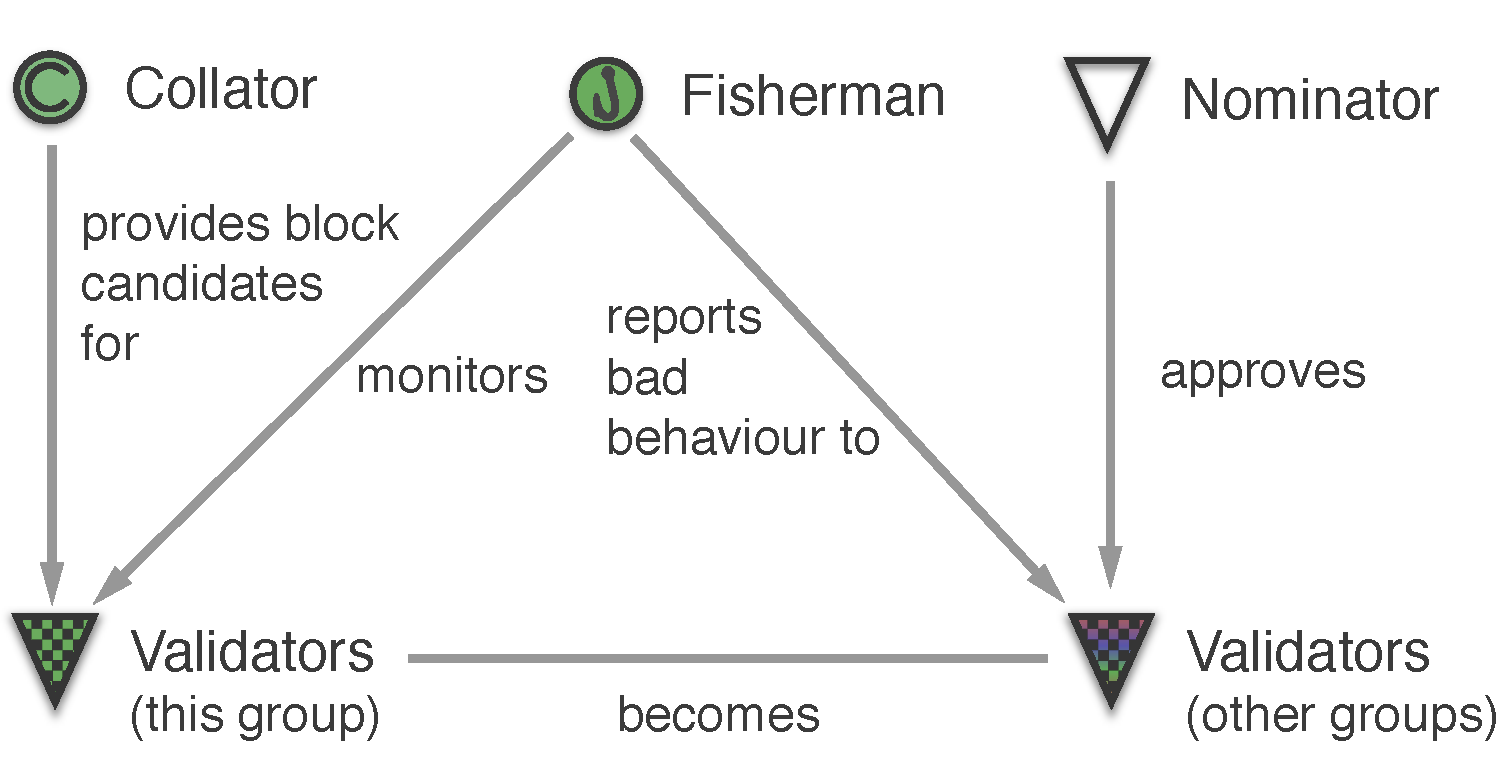
\includegraphics[width=0.96\textwidth]{Interactions.pdf}
\captionof{figure}{The interaction between the four roles of Polkadot.}
\medskip
\end{Figure}

\subsection{Validators}
\label{validators}

 A validator is the highest charge and helps seal new blocks on the Polkadot network. The validator's role is contingent upon a sufficiently high bond being deposited, though we allow other bonded parties to nominate one or more validators to act for them and as such some portion of the validator's bond may not necessarily be owned by the validator itself but rather by these nominators.

 A validator must run a relay-chain client implementation with high availability and bandwidth. At each block the node must be ready to accept the role of ratifying a new block on a nominated parachain. This process involves receiving, validating and republishing candidate blocks. The nomination is deterministic but virtually unpredictable much in advance. Since the validator cannot reasonably be expected to maintain a fully-synchronised database of all parachains, it is expected that the validator will nominate the task of devising a suggested new parachain block to a third-party, known as a collator.

 Once all new parachain blocks have been properly ratified by their appointed validator subgroups, validators must then ratify the relay-chain block itself. This involves updating the state of the transaction queues (essentially moving data from a parachain's output queue to another parachain's input queue), processing the transactions of the ratified relay-chain transaction set and ratifying the final block, including the final parachain changes.

 A validator not fulfilling their duty to find consensus under the rules of our chosen consensus algorithm is punished. For initial, unintentional failures, this is through withholding the validator's reward. Repeated failures result in the reduction of their security bond (through burning). Provably malicious actions such as double-signing or conspiring to provide an invalid block result in the loss of the entire bond (which is partially burnt but mostly given to the informant and the honest actors).

 In some sense, validators are similar to the mining pools of current PoW blockchains.

\subsection{Nominators}
\label{nominators}

 A nominator is a stake-holding party who contributes to the security bond of a validator. They have no additional role except to place risk capital and as such to signal that they trust a particular validator (or set thereof) to act responsibly in their maintenance of the network. They receive a pro-rata increase or reduction in their deposit according to the bond's growth to which they contribute.

 Together with collators, next, nominators are in some sense similar to the miners of the present-day PoW networks.

\subsection{Collators}
\label{collators}

 Transaction collators (collators for short) are parties who assist validators in producing valid parachain blocks. They maintain a ``full-node'' for a particular parachain; meaning that they retain all necessary information to be able to author new blocks and execute transactions in much the same way as miners do on current PoW blockchains. Under normal circumstances, they will collate and execute transactions to create an unsealed block, and provide it, together with a zero-knowledge proof, to one or more validators presently responsible for proposing a parachain block.

 The precise nature of the relationship between collators, nominators and validators will likely change over time. Initially, we expect collators to work very closely with validators, since there will be only a few (perhaps only one) parachain(s) with little transaction volume. The initial client implementation will include RPCs to allow a parachain collator node to unconditionally supply a (relay-chain) validator node with a provably valid parachain block. As the cost of maintaining a synced version of all such parachains increases, we expect to see additional infrastructure in place which will help separate out the duties to independent, economically-motivated, parties.

 Eventually, we expect to see collator pools who vie to collect the most transaction fees. Such collators may become contracted to serve particular validators over a period of time for an on-going share in the reward proceeds. Alternatively, ``freelance'' collators may simply create a market offering valid parachain blocks in return for a competitive share of the reward payable immediately. Similarly, decentralised nominator pools would allow multiple bonded participants to coordinate and share the duty of a validator. This ability to pool ensures open participation leading to a more decentralised system.

\subsection{Fishermen}
\label{fishermen}

 Unlike the other two active parties, fishermen are not directly related to the block-authoring process. Rather they are independent ``bounty hunters'' motivated by a large one-off reward. Precisely due to the existence of fishermen, we expect events of misbehaviour to happen seldom, and when they do only due to the bonded party being careless with secret key security, rather than through malicious intent. The name comes from the expected frequency of reward, the minimal requirements to take part and the eventual reward size.

 Fishermen get their reward through a timely proof that at least one bonded party acted illegally. Illegal actions include signing two blocks each with the same ratified parent or, in the case of parachains, helping ratify an invalid block. To prevent over-rewarding or the compromise and illicit use of a session's secret key, the base reward for providing a single validator's illegally signed message is minimal. This reward increases asymptotically as more corroborating illegal signatures from other validators are provided implying a genuine attack. The asymptote is set at 66\% following our base security assertion that at least two-thirds of the validators act benevolently.

 Fishermen are somewhat similar to ``full nodes'' in present-day blockchain systems that the resources needed are relatively small and the commitment of stable uptime and bandwidth is not necessary. Fishermen differ in so much as they must post a small bond. This bond prevents sybil attacks from wasting validators' time and compute resources. It is immediately withdrawable, probably no more than the equivalent of a few dollars and may lead to reaping a hefty reward from spotting a misbehaving validator.

%\begin{itemize}
%\item DELEGATORS vote for validators
%\item VALIDATORS validate relay-chain
%\item CHAIN-SPECIFIC SUB-GROUP VALIDATORS verify parachain transition candidate(s), ratify parachain block
%\item EACH CHAIN-SPECIFIC SUB-GROUP VALIDATOR validates collator's parachain block, suggests, votes (or, in relay-chain case) collates relay-chain transactions, suggests, votes
%\item COLLATOR collates parachain transactions, executes, provides Merkle-proof of parachain transition \& block
%\item FISHERMEN check the parachain blocks are valid, reporting invalid behaviour for reward
%\end{itemize}

\section{Design Overview}\label{design-overview}

 This section is intended to give a brief overview of the system as a whole. A more thorough exploration of the system is given in the section following it.

\begin{figure*}
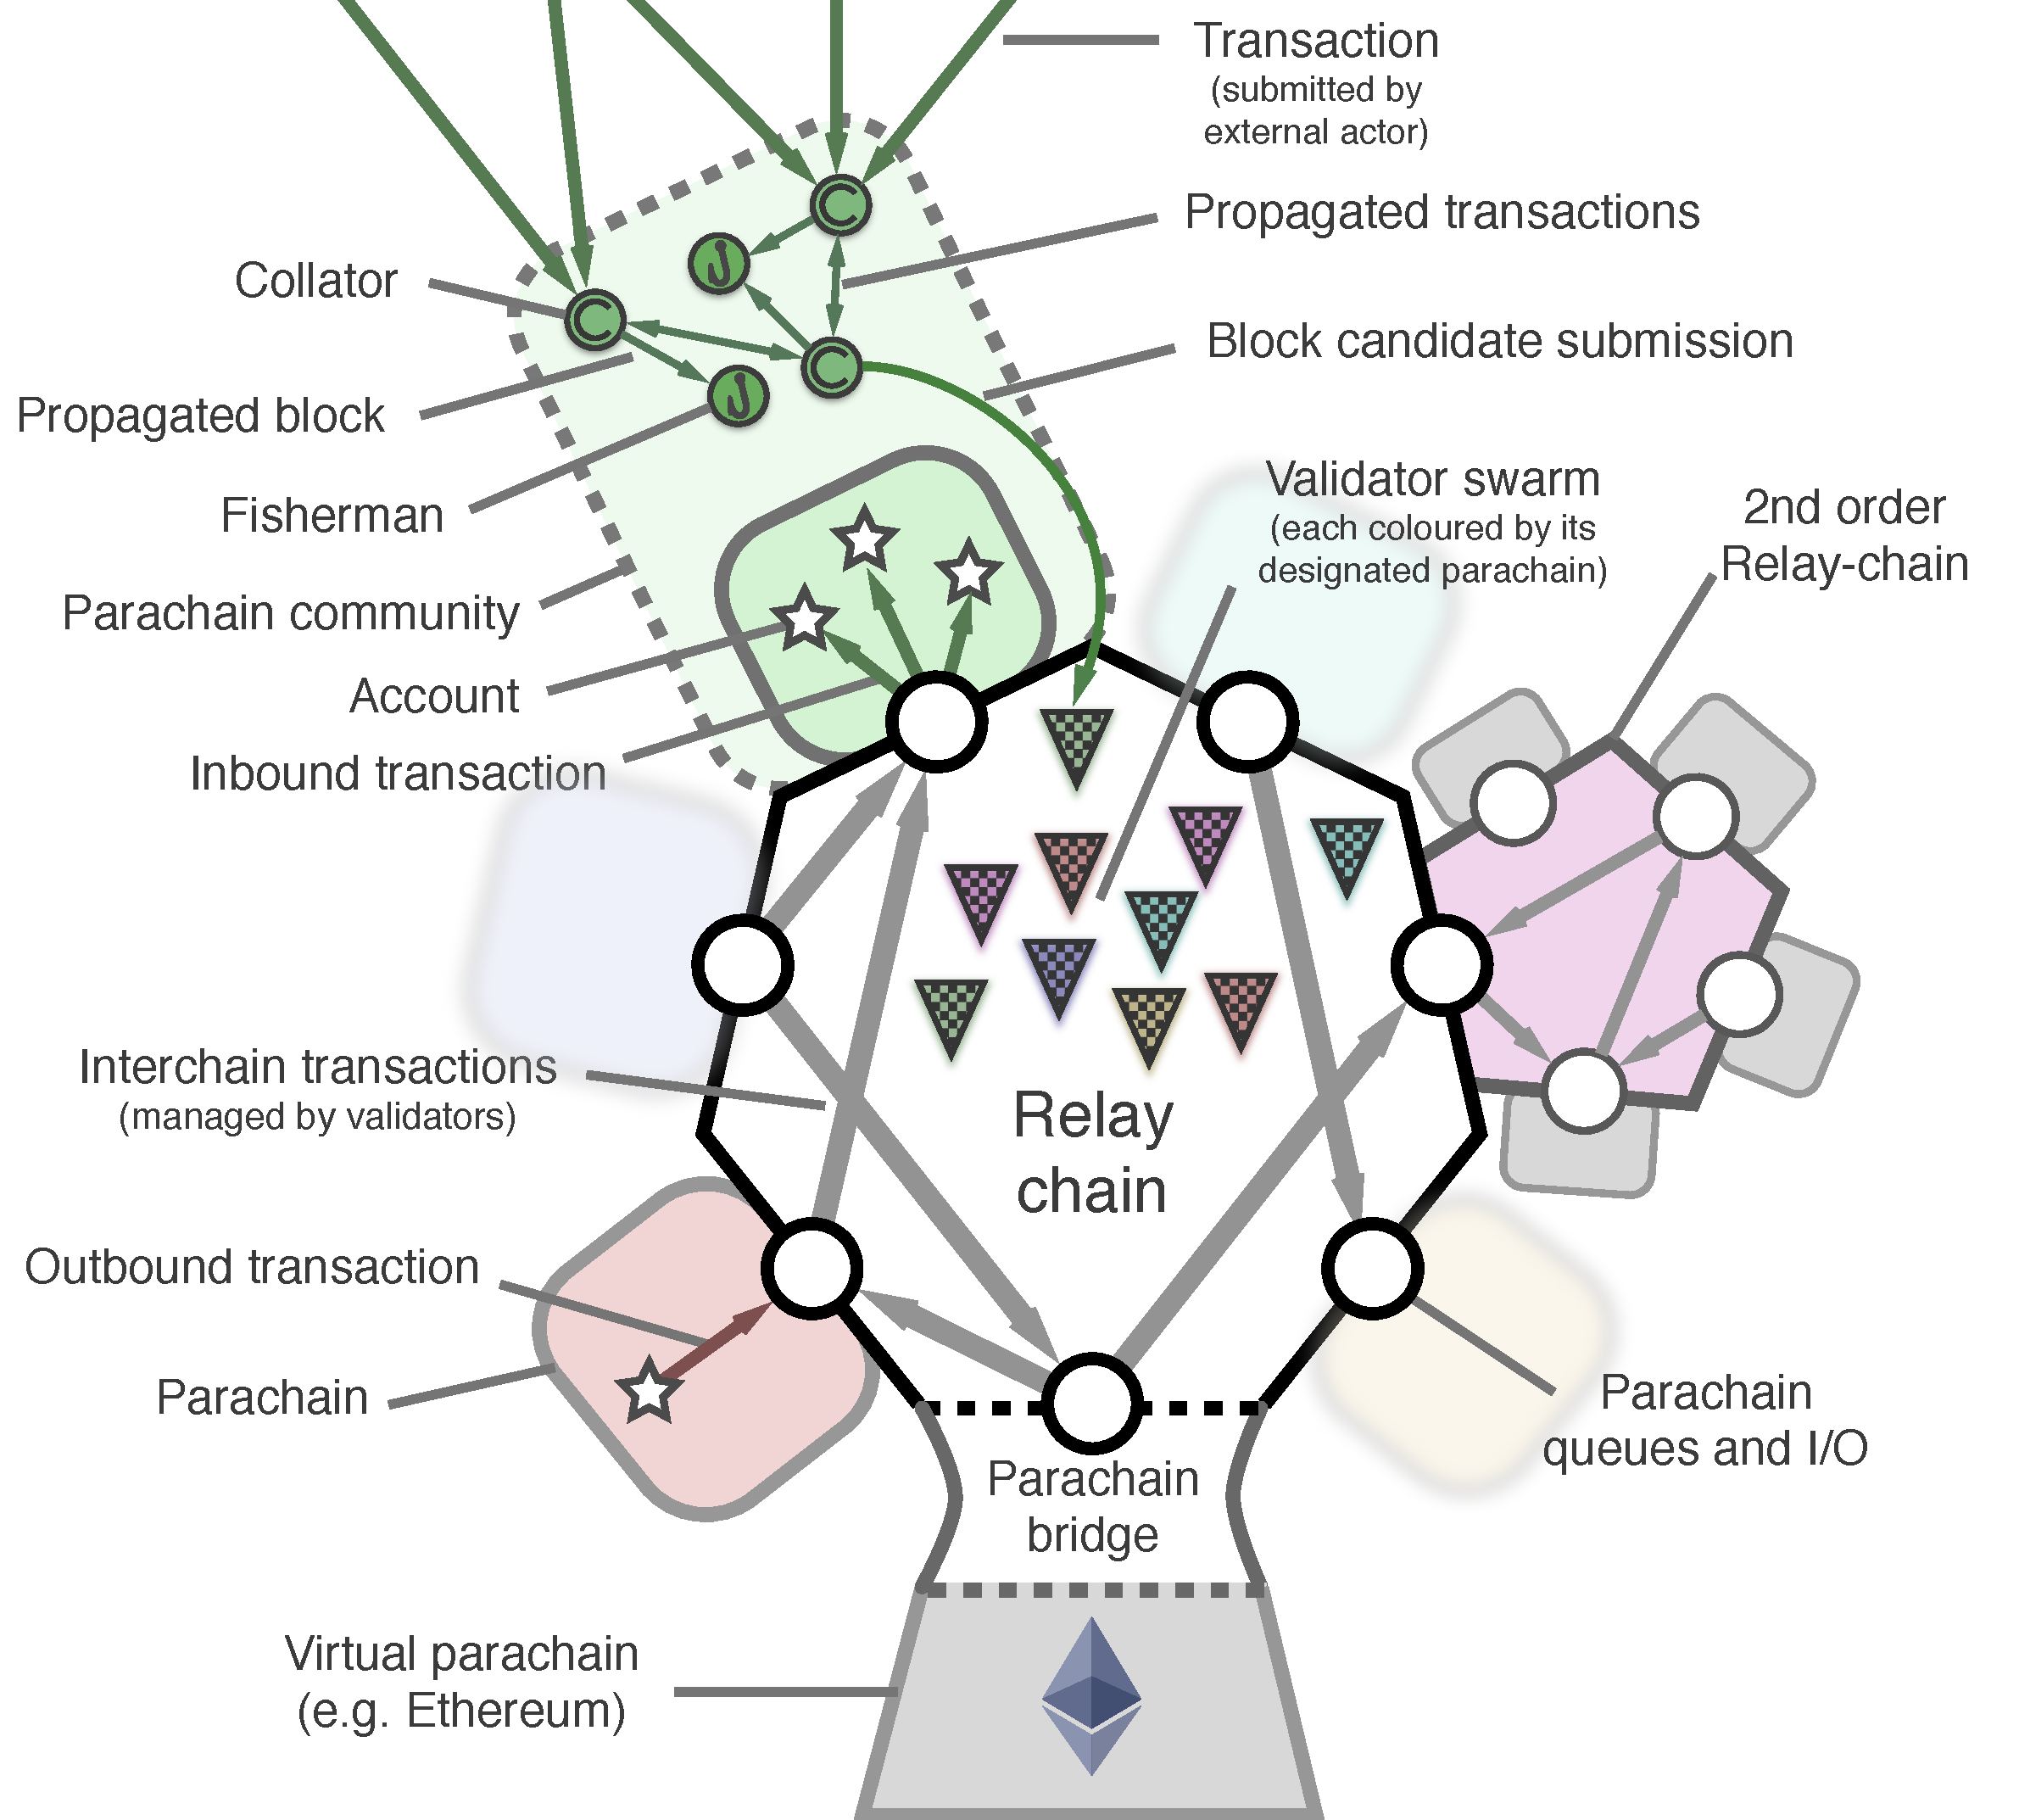
\includegraphics[width=12cm]{Overall.pdf}
\caption{A summary schematic of the Polkadot system. This shows collators collecting and propagating user-transactions, as well as propagating block candidates to fishermen and validators. It also shows how an account can post a transaction which is carried out of its parachain, via the relay-chain and on into another parachain where it can be interpreted as a transaction to an account there.}
\end{figure*}

\subsection{Consensus}\label{consensus}

 On the relay-chain, Polkadot achieves low-level consensus over a set of mutually agreed valid blocks through a modern asynchronous Byzantine fault-tolerant (BFT) algorithm. The algorithm will be inspired by the simple Tendermint\cite{kwon2014tendermint} and the substantially more involved HoneyBadgerBFT\cite{miller2016honey}. The latter provides an efficient and fault-tolerant consensus over an arbitrarily defective network infrastructure, given a set of mostly benign authorities or \emph{validators}.

 For a proof-of-authority (PoA) style network, this alone would be sufficient, however Polkadot is imagined to be also deployable as a network in a fully open and public situation without any particular organisation or trusted authority required to maintain it. As such we need a means of determining a set of validators and incentivising them to be honest. For this we utilise PoS based selection criteria.

\subsection{Proving the Stake}\label{proving-the-stake}

 We assume that the network will have some means of measuring how much ``stake'' any particular account has. For ease of comparison to pre-existing systems, we will call the unit of measurement ``tokens''. Unfortunately the term is less than ideal for a number of reasons, not least that being simply a scalar value associated with an account, there is no notion of individuality.

 We imagine validators be elected, infrequently (at most once per day but perhaps as seldom as once per quarter), through a \textit{Nominated Proof-of-Stake} (\textit{NPoS}) scheme. Incentivisation can happen through a pro-rata allocation of funds coming from a token base expansion (up to 100\% per year, though more likely around 10\%) together with any transaction fees collected. While monetary base expansion typically leads to inflation, since all token owners would have a fair opportunity at participation, no token-holder would need to suffer a reduction in value of their holdings over time provided they were happy to take a role in the consensus mechanism. A particular proportion of tokens would be targeted for the staking process; the effective token base expansion would be adjusted through a market-based mechanism to reach this target.

 Validators are bonded heavily by their stakes; exiting validators' bonds remain in place long after the validators' duties cease (perhaps around 3 months). This long bond-liquidation period allows future misbehaviour to be punished up until the periodic checkpointing of the chain. Misbehaviour results in punishment, such as reduction of reward or, in cases which intentionally compromise the network's integrity, the validator losing some or all of its stake to other validators, informants or the stakeholders as a whole (through burning). For example, a validator who attempts to ratify both branches of a fork (sometimes known as a ``short-range'' attack) may be identified and punished in the latter way.

Long-range ``nothing-at-stake'' attacks\footnote{Such an attack is where the adversary forges an entirely new chain of history from the genesis block onwards. Through controlling a relatively insignificant portion of stake at the offset, they are able to incrementally increase their portion of the stake relative to all other stakeholders as they are the only active participants in their alternative history. Since no intrinsic physical limitation exists on the creation of blocks (unlike PoW where quite real computational energy must be spent), they are able to craft a chain longer than the real chain in a relatively short timespan and potentially make it the longest and best, taking over the canonical state of the network.} are circumvented through a simple ``checkpoint'' latch which prevents a dangerous chain-reorganisation of more than a particular chain-depth. To ensure newly-syncing clients are not able to be fooled onto the wrong chain, regular ``hard forks'' will occur (of at most the same period of the validators' bond liquidation) that hard-code recent checkpoint block hashes into clients. This plays well with a further footprint-reducing measure of ``finite chain length'' or periodic reseting of the genesis-block.

\subsection{Parachains and Collators}\label{parachains-and-collators}

 Each parachain gets similar security affordances to the relay-chain: the parachains' headers are sealed within the relay-chain block ensuring no reorganisation, or ``double-spending'', is possible following confirmation. This is a similar security guarantee to that offered by Bitcoin's side-chains and merge-mining. Polkadot, however, also provides strong guarantees that the parachains' state transitions are valid. This happens through the set of validators being cryptographically randomly segmented into subsets; one subset per parachain, the subsets potentially differing per block. This setup generally implies that parachains' block times will be at least as long as that of the relay-chain. The specific means of determining the partitioning is outside the scope of this document but would likely be based either around a commit-reveal framework similar to the \textit{RanDAO}\cite{randao} or use data combined from previous blocks of each parachain under a cryptographically secure hash.

 Such subsets of validators are required to provide a parachain block candidate which is guaranteed valid (on pain of bond confiscation). Validity revolves around two important points; firstly that it is intrinsically valid---that all state transitions were executed faithfully and that all external data referenced (i.e. transactions) is valid for inclusion. Secondly, that any data which is extrinsic to its candidate, such as those external transactions, has sufficiently high availability so that participants are able to download it and execute the block manually.\footnote{Such a task might be shared between validators or could become the designate task of a set of heavily bonded validators known as \textit{availability guarantors}.} Validators may provide only a ``null'' block containing no external ``transactions'' data, but may run the risk of getting a reduced reward if they do. They work alongside a parachain gossip protocol with \emph{collators}---individuals who collate transactions into blocks and provide a non-interactive, zero-knowledge proof that the block constitutes a valid child of its parent (and taking any transaction fees for their trouble).

 It is left to parachain protocols to specify their own means of spam-prevention: there is no fundamental notion of ``compute-resource metering'' or ``transaction fee'' imposed by the relay-chain. There is also no direct enforcement on this by the relay-chain protocol (though it is unlikely that the stakeholders would choose to adopt a parachain which didn't provide a decent mechanism). This is an explicit nod to the possibility of chains unlike Ethereum, \eg a Bitcoin-like chain which has a much simpler fee model or some other, yet-to-be-proposed spam-prevention model.

 Polkadot's relay-chain itself will probably exist as an Ethereum-like accounts and state chain, possibly an EVM-derivative. Since the relay-chain nodes will be required to do substantial other processing, transaction throughput will be minimised partly through large transaction fees and, should our research models require, a block size limit.

\subsection{Interchain Communication}
\label{interchain-communication}

 The critical final ingredient of Polkadot is interchain communication. Since parachains can have some sort of information channel between them, we allow ourselves to consider Polkadot a scalable multi-chain. In the case of Polkadot, the communication is as simple as can be: transactions executing in a parachain are (according to the logic of that chain) able to effect the dispatch of a transaction into a second parachain or, potentially, the relay-chain. Like external transactions on production blockchains, they are fully asynchronous and there is no intrinsic ability for them to return any kind of information back to its origin.

\begin{Figure}
\medskip
\centering
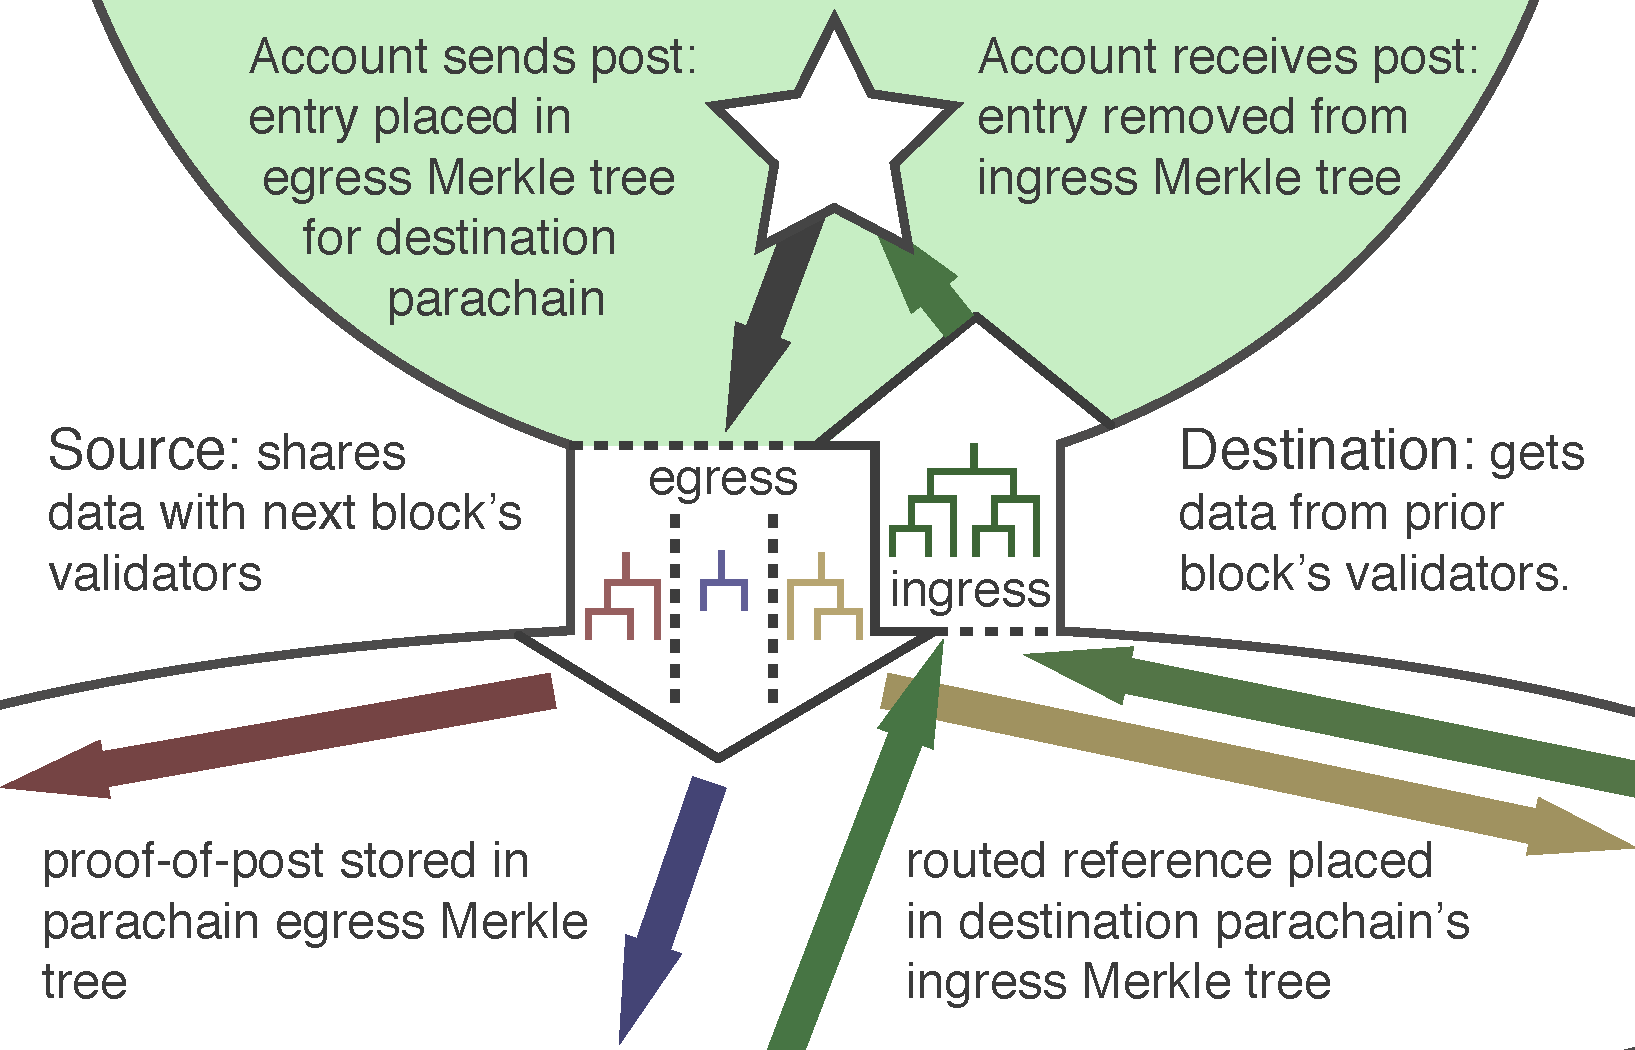
\includegraphics[width=0.96\textwidth]{Queues.pdf}
\captionof{figure}{A basic schematic showing the main parts of routing for posted transactions ("posts").}
\medskip
\end{Figure}

 To ensure minimal implementation complexity, minimal risk and minimal straight-jacketing of future parachain architectures, these interchain transactions are effectively indistinguishable from standard externally-signed transactions. The transaction has an origin segment, providing the ability to identify a parachain, and an address which may be of arbitrary size. Unlike common current systems such as Bitcoin and Ethereum, interchain transactions do not come with any kind of ``payment'' of fee associated; any such payment must be managed through negotiation logic on the source and destination parachains. A system such as that proposed for Ethereum's Serenity release\cite{buterin2016serenity} would be a simple means of managing such a cross-chain resource payment, though we assume others may come to the fore in due course.

 Interchain transactions are resolved using a simple queuing mechanism based around a Merkle tree to ensure fidelity. It is the task of the relay-chain maintainers to move transactions on the output queue of one parachain into the input queue of the destination parachain. The passed transactions get referenced on the relay-chain, however are not relay-chain transactions themselves. To prevent a parachain from spamming another parachain with transactions, for a transaction to be sent, it is required that the destination's input queue be not too large at the time of the end of the previous block. If the input queue is too large after block processing, then it is considered ``saturated'' and no transactions may be routed to it within subsequent blocks until reduced back below the limit. These queues are administered on the relay-chain allowing parachains to determine each other's saturation status; this way a failed attempt to post a transaction to a stalled destination may be reported synchronously. (Though since no return path exists, if a secondary transaction failed for that reason, it could not be reported back to the original caller and some other means of recovery would have to take place.)

\subsection{Polkadot and Ethereum}\label{disparity-and-ethereum}

 Due to Ethereum's Turing completeness, we expect there is ample opportunity for Polkadot and Ethereum to be interoperable with each other, at least within some easily deducible security bounds. In short, we envision that transactions from Polkadot can be signed by validators and then fed into Ethereum where they can be interpreted and enacted by a transaction-forwarding contract. In the other direction, we foresee the usage of specially formatted logs (events) coming from a ``break-out contract'' to allow a swift verification that a particular message should be forwarded.

\subsubsection{Polkadot to Ethereum}\label{disparity-to-ethereum}

 Through the choice of a BFT consensus mechanism with validators formed from a set of stakeholders determined through an approval voting mechanism, we are able to get a secure consensus with an infrequently changing and modest number of validators. In a system with a total of 144 validators, a block time of 4 seconds and a 900-block finality (allowing for malicious behaviour such as double-votes to be reported, punished and repaired), the validity of a block can reasonably be considered proven through as little as 97 signatures (two-thirds of 144 plus one) and a following 60-minute verification period where no challenges are deposited.

 Ethereum is able to host a ``break-in contract'' which can maintain the 144 signatories and be controlled by them. Since elliptic curve digital signature (ECDSA) recovery takes only 3,000 gas under the EVM, and since we would likely only want the validation to happen on a super-majority of validators (rather than full unanimity), the base cost of Ethereum confirming that an instruction was properly validated as coming from the Polkadot network would be no more than 300,000 gas---a mere 6\% of the total block gas limit at 5.5M. Increasing the number of validators (as would be necessary for dealing with dozens of chains) inevitably increases this cost, however it is broadly expected for Ethereum's transaction bandwidth to grow over time as the technology matures and infrastructure improves. Together with the fact that not all validators need to be involved (\eg only the highest staked validators may be called upon for such a task) the limits of this mechanism extend reasonably well.

 Assuming a daily rotation of such validators (which is fairly conservative---weekly or even monthly may be acceptable), then the cost to the network of maintaining this Ethereum-forwarding bridge would be around 540,000 gas per day or, at present gas prices, \$45 per year. A basic transaction forwarded alone over the bridge would cost around \$0.11; additional contract computation would cost more, of course. By buffering and bundling transactions together, the break-in authorisation costs can easily be shared, reducing the cost per transaction substantially; if 20 transactions were required before forwarding, then the cost for forwarding a basic transaction would fall to around \$0.01.
 
 One interesting, and cheaper, alternative to this multi-signature contract model would be to use threshold signatures in order to achieve the multi-lateral ownership semantics. While threshold signature schemes for ECDSA are computationally expensive, those for other schemes such as Schnorr signatures are very reasonable. Ethereum plans to introduce primitives which would make such schemes cheap to use in the upcoming Metropolis hard-fork. If such a means were able to be utilised, the gas costs for forwarding a Polkadot transaction into the Ethereum network would be dramatically reduced to a near zero overhead over and above the basic costs for validating the signature and executing the underlying transaction.

 In this model, Polkadot's validator nodes would have to do little other than sign messages. To get the transactions actually routed onto the Ethereum network, we assume either validators themselves would also reside on the Ethereum network or, more likely, that small bounties be offered to the first actor who forwards the message on to the network (the bounty could trivially be paid to the transaction originator).

\subsubsection{Ethereum to Polkadot}\label{ethereum-to-disparity}

 Getting transactions to be forwarded from Ethereum to Polkadot uses the simple notion of logs. When an Ethereum contract wishes to dispatch a transaction to a particular parachain of Polkadot, it need simply call into a special ``break-out contract''. The break-out contract would take any payment that may be required and issue a logging instruction so that its existence may be proven through a Merkle proof and an assertion that the corresponding block's header is valid and canonical.

 Of the latter two conditions, validity is perhaps the most straightforward to prove. In principle, the only requirement is for each Polkadot node needing the proof (i.e.~appointed validator nodes) to be running a fully synchronised instance of a standard Ethereum node. Unfortunately, this is itself a rather heavy dependency. A more lightweight method would be to use a simple proof that the header was evaluated correctly through supplying only the part of Ethereum's state trie needed to properly execute the transactions in the block and check that the logs (contained in the block receipt) are valid. Such ``SPV-like''\footnote{SPV refers to Simplified Payment Verification in Bitcoin and describes a method for clients to verify transactions while keeping only a copy of all blocks headers of the longest PoW chain.} proofs may yet require a substantial amount of information; conveniently, they would typically not be needed at all: a bond system inside Polkadot would allow bonded third-parties to submit headers at the risk of losing their bond should some other third-party (such as a ``fisherman'', see \ref{bond-confiscationburning}) provide a proof that the header is invalid (specifically that the state root or receipt roots were impostors).

 On a non-finalising PoW network like Ethereum, the canonicality is impossible to proof conclusively. To address this, applications that attempt to rely on any kind of chain-dependent cause-effect wait for a number of ``confirmations'', or until the dependent transaction is at some particular depth within the chain. On Ethereum, this depth varies from 1 block for the least valuable transactions with no known network issues to 1200 blocks as was the case during the initial Frontier release for exchanges. On the stable ``Homestead'' network, this figure sits at 120 blocks for most exchanges, and we would likely take a similar parameter.
 % is there a reference for the 120 block statement?

 So we can imagine our Polkadot-side Ethereum-interface to have some simple functions: to be able to accept a new header from the Ethereum network and validate the PoW, to be able to accept some proof that a particular log was emitted by the Ethereum-side break-out contract for a header of sufficient depth (and forward the corresponding message within Polkadot) and finally to be able to accept proofs that a previously accepted but not-yet-enacted header contains an invalid receipt root.

 To actually get the Ethereum header data itself (and any SPV proofs or validity/canonicality refutations) into the Polkadot network, an incentivisation for forwarding data is needed. This could be as simple as a payment (funded from fees collected on the Ethereum side) paid to anyone able to forward a useful block whose header is valid. Validators would be called upon to retain information relating to the last few thousand blocks in order to be able to manage forks, either through some protocol-intrinsic means or through a contract maintained on the relay chain.

\subsection{Polkadot and Bitcoin}\label{disparity-and-bitcoin}

 Bitcoin interoperation presents an interesting challenge for Polkadot: a so-called ``two-way peg'' would be a useful piece of infrastructure to have on the side of both networks. However, due to the limitations of Bitcoin, providing such a peg securely is a non-trivial undertaking. Delivering a transaction from Bitcoin to Polkadot can in principle be done with a process similar to that for Ethereum; a ``break-out address'' controlled in some way by the Polkadot validators could receive transferred tokens (and data sent alongside them). SPV proofs could be provided by incentivised oracles and, together with a confirmation period, a bounty given for identifying non-canonical blocks implying the transaction has been ``double-spent''. Any tokens then owned in the ``break-out address'' would then, in principle, be controlled by those same validators for later dispersal.

 The problem however is how the deposits can be securely controlled from a rotating validator set. Unlike Ethereum which is able to make arbitrary decisions based upon combinations of signatures, Bitcoin is substantially more limited, with most clients accepting only multi-signature transactions with a maximum of 3 parties. Extending this to 36, or indeed thousands as might ultimately be desired, is impossible under the current protocol. One option is to alter the Bitcoin protocol to enable such functionality, however so-called ``hard forks'' in the Bitcoin world are difficult to arrange judging by recent attempts. One possibility is the use of threshold signatures, cryptographic schemes to allow a singly identifiable public key to be effectively controlled by multiple secret ``parts'', some or all of which must be utilised to create a valid signature. Unfortunately, threshold signatures compatible with Bitcoin's ECDSA are computationally expensive to create and of polynomial complexity. Other schemes such a Schnorr signatures provide far lower costs, however the timeline on which they may be introduced into the Bitcoin protocol is uncertain.

 Since the ultimate security of the deposits rests with a number of bonded validators, one other option is to reduce the multi-signature key-holders to only a heavily bonded subset of the total validators such that threshold signatures become feasible (or, at worst, Bitcoin's native multi-signature is possible). This of course reduces the total amount of bonds that could be deducted in reparations should the validators behave illegally, however this is a graceful degradation, simply setting an upper limit of the amount of funds that can securely run between the two networks (or indeed, on the \% losses should an attack from the validators succeed).

 As such we believe it not unrealistic to place a reasonably secure Bitcoin interoperability ``virtual parachain'' between the two networks, though nonetheless a substantial effort with an uncertain timeline and quite possibly requiring the cooperation of the stakeholders within that network.

\section{Protocol in Depth}\label{protocol-in-depth}

 The protocol can be roughly broken down into three parts: the consensus mechanism, the parachain interface and interchain transaction routing.

\subsection{Relay-chain Operation}\label{relay-chain-operation}

 The relay-chain will likely be a chain broadly similar to Ethereum in that it is state-based with the state mapping address to account information, mainly balances and (to prevent replays) a transaction counter. Placing accounts here fulfils one purpose: to provide accounting for which identity possesses what amount of stake in the system.\footnote{As a means of representing the amount a given holder is responsible for the overall security of the system, these stake accounts will inevitably encode some economic value. However, it should be understood that since there is no intention that such values be used in any way for the purpose of exchanging for real-world goods and services, it should be accordingly noted that the tokens not be likened to currency and as such the relay-chain retain its nihilistic philosophy regarding applications.} There will be notable differences, though:

\begin{itemize}
\item Contracts cannot be deployed through transactions; following from the desire to avoid application functionality on the relay-chain, it will not support public deployment of contracts.
\item Compute resource usage (``gas'') is not accounted; since the only functions available for public usage will be fixed, the rationale behind gas accounting no longer holds. As such, a flat fee will apply in all cases, allowing for more performance from any dynamic code execution that may need to be done and a simpler transaction format.
\item Special functionality is supported for listed contracts that allows for auto-execution and network-message outputs.
\end{itemize}

 In the event that the relay-chain has a VM and it be based around the EVM, it would have a number of modifications to ensure maximal simplicity. It would likely have a number of built-in contracts (similar to those at addresses 1-4 in Ethereum) to allow for platform-specific duties to be managed including a consensus contract, a validator contract and a parachain contract.

 If not the EVM, then a WebAssembly\cite{webassembly} (wasm) back-end is the most likely alternative; in this case the overall structure would be similar, but there would be no need for the built-in contracts with Wasm being a viable target for general purpose languages rather than the immature and limited languages for the EVM.

 Other likely deviations from the present Ethereum protocol are quite possible, for example a simplification of the transaction-receipt format allowing for the parallel execution of non-conflicting transactions within the same block, as proposed for the Serenity series of changes.

 It is possible, though unlikely, that a Serenity-like ``pure'' chain be deployed as the relay-chain, allowing for a particular contract to manage things like the staking token balances rather than making that a fundamental part of the chain's protocol. At present, we feel it is unlikely this will offer a sufficiently great protocol simplification to be worth the additional complexity and uncertainty involved in developing it.

 There are a number of small pieces of functionality required for administrating the consensus mechanism, validator set, validation mechanism and parachains. These could be implemented together under a monolithic protocol. However, for reasons of auguring modularity, we describe these as ``contracts'' of the relay-chain. This should be taken to mean that they are objects (in the sense of object-orientated programming) managed by the relay-chain's consensus mechanism, but not necessarily that they are defined as programs in EVM-like opcodes, nor even that they be individually addressable through the account-system.

\subsection{Staking Contract}
\label{staking-contract}

 This contract maintains the validator set. It manages:

\begin{itemize}
\tightlist
\item which accounts are currently validators;
\item which are available to become validators at short notice;
\item which accounts have placed stake nominating to a validator;
\item properties of each including staking volume, acceptable payout-rates and addresses and short-term (session) identities.
\end{itemize}

 It allows an account to register a desire to become a bonded validator (along with its requirements), to nominate to some identity, and for preexisting bonded validators to register their desire to exit this status. It also includes the machinery itself for the validation and canonicalisation mechanism.

\subsubsection{Stake-token Liquidity}
\label{stake-token-liquidity}

 It is generally desirable to have as much of the total staking tokens as possible to be staked within the network maintenance operations since this directly ties the network security to the overall ``market capitalisation'' of the staking token. This can easily be incentivised through inflating the currency and handing out the proceeds to those who participate as validators. However, to do so presents a problem: if the token is locked in the Staking Contract under punishment of reduction, how can a substantial portion remain sufficiently liquid in order to allow price discovery?

 One answer to this is allowing a straight-forward derivative contract, securing fungible tokens on an underlying staked token. This is difficult to arrange in a trust-free manner. Furthermore, these derivative tokens cannot be treated equally for the same reason that different Eurozone government's bonds are not fungible: there is a chance of the underlying asset failing and becoming worthless. With Eurozone governments, there could be a default. With validator-staked tokens, the validator may act maliciously and be punished.

 Keeping with our tenets, we elect for the simplest solution: not all tokens be staked. This would mean that some proportion (perhaps 20\%) of tokens will forcibly remain liquid. Though this is imperfect from a security perspective, it is unlikely to make a fundamental difference in the security of the network; 80\% of the reparations possible from bond-confiscations would still be able to be made compared to the ``perfect case'' of 100\% staking.

 The ratio between staked and liquid tokens can be targeted fairly simply through a reverse auction mechanism. Essentially, token holders interested in being a validator would each post an offer to the staking contract stating the minimum payout-rate that they would require to take part. At the beginning of each session (sessions would happen regularly, perhaps as often as once per hour) the validator slots would be filled according to each would-be validator's stake and payout rate. One possible algorithm for this would be to take those with the lowest offers who represent a stake no higher than the total stake targeted divided by the number of slots and no lower than a lower-bound of half that amount. If the slots cannot be filled, the lower bound could be repeatedly reduced by some factor in order to satisfy.

\subsubsection{Nominating}
\label{nominating}

 It is possible to trustlessly nominate ones staking tokens to an active validator, giving them the responsibility of validators duties. Nominating works through an approval-voting system. Each would-be nominator is able to post an instruction to the staking contract expressing one or more validator identities under whose responsibility they are prepared to entrust their bond.

 Each session, nominators' bonds are dispersed to be represented by one or more validators. The dispersal algorithm optimises for a set of validators of equivalent total bonds. Nominators' bonds become under the effective responsibility of the validator and gain interest or suffer a punishment-reduction accordingly.

\subsubsection{Bond Confiscation/Burning}
\label{bond-confiscationburning}

 Certain validator behaviour results in a punitive reduction of their bond. If the bond is reduced below the allowable minimum, the session is prematurely ended and another started. A non-exhaustive list of punishable validator misbehaviour includes:

\begin{itemize}
\item Being part of a parachain group unable to provide consensus over the validity of a parachain block;
\item actively signing for the validity of an invalid parachain block;
\item inability to supply egress payloads previously voted as available;
\item inactivity during the consensus process;
\item validating relay-chain blocks on competing forks.
\end{itemize}

 Some cases of misbehaviour threaten the network's integrity (such as signing invalid parachain blocks and validating multiple sides of a fork) and as such result in effective exile through the total reduction of the
bond. In other, less serious cases (\eg~inactivity in the consensus process) or cases where blame cannot be precisely allotted (being part of an ineffective group), a small portion of the bond may instead be fined. In the latter case, this works well with sub-group churn to ensure that malicious nodes suffer substantially more loss than the collaterally-damaged benevolent nodes.

In some cases (\eg~multi-fork validation and invalid sub-block signing) validators cannot themselves easily detect each others' misbehaviour since constant verification of each parachain block would be too arduous a task. Here it is necessary to enlist the support of parties external to the validation process to verify and report such misbehaviour. The parties get a reward for reporting such activity; their term, ``fishermen'' stems from the unlikeliness of such a reward.

 Since these cases are typically very serious, we envision that any rewards can easily be paid from the confiscated bond. In general we prefer to balance burning (\ie reduction to nothing) with reallocation, rather than attempting wholesale reallocation. This has the effect of increasing the overall value of the token, compensating the network in general to some degree rather than the specific party involved in discovery. This is mainly as a safety mechanism: the large amounts involved could lead to extreme and acute behaviour incentivisation were they all bestowed on a single target.

 In general, it is important that the reward is sufficiently large to make verification worthwhile for the network, yet not so large as to offset the costs of fronting a well-financed, well-orchestrated "industrial-level" criminal hacking attack on some unlucky validator to force misbehaviour.

 In this way, the amount claimed should generally be no greater than the direct bond of the errant validator, lest a perverse incentive arise of misbehaving and reporting oneself for the bounty. This can be combated either explicitly through a minimum direct bond requirement for being a validator or implicitly by educating nominators that validators with little bonds deposited have no great incentive to behave well.

\subsection{Parachain Registry}
\label{parachain-registry}

 Each parachain is defined in this registry. It is a relatively simple database-like construct and holds both static and dynamic information on each chain.

 Static information includes the chain index (a simple integer), along with the validation protocol identity, a means of distinguishing between the different classes of parachain so that the correct validation algorithm can be run by validators consigned to putting forward a valid candidate. An initial proof-of-concept would focus on placing the new validation algorithms into clients themselves, effectively requiring a hard fork of the protocol each time an additional class of chain were added. Ultimately, though, it may be possible to specify the validation algorithm in a way both rigorous and efficient enough that clients are able to effectively work with new parachains without a hard-fork. One possible avenue to this would be to specify the parachain validation algorithm in a well-established, natively-compiled, platform-neutral language such as WebAssembly. Additional research is necessary to determine whether this is truly feasible, however if so, it could bring with it the tremendous advantage of banishing hard-forks for good.

 Dynamic information includes aspects of the transaction routing system that must have global agreement such as the parachain's ingress queue (described in section \ref{interchain-transaction-routing}).

 The registry is able to have parachains added only through full referendum voting; this could be managed internally but would more likely be placed in an external referendum contract in order to facilitate re-usage under more general governance components. The parameters to voting requirements (\eg~any quorum required, majority required) for registration of additional chains and other, less formal system upgrades will be set out in a ``master constitution'' but are likely to follow a fairly traditional path, at least initially. The precise formulation is out of scope for the present work, but \eg~a two thirds super-majority to pass with more than one third of total system stake voting positively may be a sensible starting point.

 Additional operations include the suspension and removal of parachains. Suspension would hopefully never happen, however it is designed to be a safeguard least there be some intractable problem in a parachain's validation system. The most obvious instance where it might be needed is a consensus-critical difference between implementations leading validators to be unable to agree on validity or blocks. Validators would be encouraged to use multiple client implementations in order that they are able to spot such a problem prior to bond confiscation.

 Since suspension is an emergency measure, it would be under the auspices of the dynamic validator-voting rather than a referendum. Re-instating would be possible both from the validators or a referendum.

 The removal of parachains altogether would come only after a referendum and with which would be required a substantial grace period to allow an orderly transition to either a standalone chain or to become part of some other consensus-system. The grace period would likely be of the order of months and is likely to be set out on a per-chain basis in the parachain registry in order that different parachains can enjoy different grace periods according to their need.

\subsection{Sealing Relay Blocks}
\label{sealing-relay-blocks}

 Sealing refers, in essence, to the process of canonicalisation; that is, a basic data transform which maps the original into something fundamentally singular and meaningful. Under a PoW chain, sealing is effectively a synonym for \emph{mining}. In our case, it involves the collection of signed statements from validators over the validity, availability and canonicality of a particular relay-chain block and the parachain blocks that it represents.

 The mechanics of the underlying BFT consensus algorithm is out of scope for the present work. We will instead describe it using a primitive which assumes a consensus-creating state-machine. Ultimately we expect to be inspired by a number of promising BFT consensus algorithms in the core; Tangaora\cite{copeland2016tangaroa} (a BFT variant of Raft\cite{ongaro2014search}), Tendermint\cite{kwon2014tendermint} and HoneyBadgerBFT\cite{miller2016honey}. The algorithm will have to reach an agreement on multiple parachains in parallel, thus differing from the usual blockchain consensus mechanisms. We assume that once consensus is reached, we are able to record the consensus in an irrefutable proof which can be provided by any of the participants to it. We also assume that misbehaviour within the protocol can be generally reduced to a small group containing misbehaving participants to minimise the collateral damage when dealing out punishment.\footnote{Existing PoS-based BFT consensus schemes such as Tendermint BFT and the original Slasher fulfill these assertions.}

 The proof, which takes the form of our signed statements, is placed in the relay-chain block's header together with certain other fields not least the relay-chain's state-trie root and transaction-trie root.

 The sealing process takes place under a single consensus-generating mechanism addressing both the relay-chain's block and the parachains' blocks which make up part of the relay's content: parachains are not separately ``committed'' by their sub-groups and then collated later. This results in a more complex process for the relay-chain, but allows us to complete the entire system's consensus in a single stage, minimising latency and allowing for quite complex data-availability requirements which are helpful for the routing process below.
 
 % a visual example  would be very useful here

 The state of each participant's consensus machine may be modelled as a simple (2-dimensional) table. Each participant (validator) has a set of information, in the form of signed-statements (``votes'') from other participants, regarding each parachain block candidate as well the relay-chain block candidate. The set of information is two pieces of data:

\begin{description}
\item[Availability] does this validator have egress transaction-post information from this block so they are able to properly validate parachain candidates on the following block? They may vote either 1(known) or 0 (not yet known). Once they vote 1, they are committed to voting similarly for the rest of this process. Later votes that do not respect this are grounds for punishment.
\item[Validity] is the parachain block valid and is all externally-referenced data (e.g. transactions) available? This is only relevant for validators assigned to the parachain on which they are voting. They may vote either 1 (valid), -1 (invalid) or 0 (not yet known). Once they vote non-zero, they are committed to voting this way for the rest of the process. Later votes that do not respect this are grounds for punishment.
\end{description}

 All validators must submit votes; votes may be resubmitted, qualified by the rules above. The progression of consensus may be modelled as multiple standard BFT consensus algorithms over each parachain happening in parallel. Since these are potentially thwarted by a relatively small minority of malicious actors being concentrated in a single parachain group, the overall consensus exists to establish a backstop, limiting the worst-case scenario from deadlock to merely one or more void parachain blocks (and a round of punishment for those responsible).

 The basic rules for validity of the individual blocks (that allow the total set of validators as a whole to come to consensus on it becoming the unique parachain candidate to be referenced from the canonical relay):

\begin{itemize}
\item must have at least two thirds of its validators voting positively and none voting negatively;
\item must have over one third validators voting positively to the availability of egress queue information.
\end{itemize}

 If there is at least one positive and at least one negative vote on validity, an exceptional condition is created and the whole set of validators must vote to determine if there are malicious parties or if there is an accidental fork. Aside from valid and invalid, a third kind of votes are allowed, equivalent to voting for both, meaning that the node has conflicting opinions. This could be due to the node's owner running multiple implementations which do not agree, indicating a possible ambiguity in the protocol.

 After all votes are counted from the full validator set, if the losing opinion has at least some small proportion (to be parameterised; at most half, perhaps significantly less) of the votes of the winning opinion, then it is assumed to be an accidental parachain fork and the parachain is automatically suspended from the consensus process. Otherwise, we assume it is a malicious act and punish the minority who were voting for the dissenting opinion.

 The conclusion is a set of signatures demonstrating canonicality. The relay-chain block may then be sealed and the process of sealing the next block begun.

\subsection{Improvements for Sealing Relay Blocks}
\label{improvements-for-sealing-relay-blocks}

 While this sealing method gives strong guarantees over the system's operation, it does not scale out particularly well since every parachain's key information must have its availability guaranteed by over one-third of all validators. This means that every validator's responsibility footprint grows as more chains are added.

 While data availability within open consensus networks is essentially an unsolved problem, there are ways of mitigating the overhead placed on validator nodes. One simple solution is to realise that while validators must shoulder the \emph{responsibility} for data availability, they need not actually store, communicate or replicate the data themselves. Secondary data silos, possibly related to (or even the very same) collators who compile this data, may manage the task of guaranteeing availability with the validators providing a portion of their interest/income in payment.

 However, while this might buy some intermediate scalability, it still doesn't help the underlying problem; since adding more chains will in general require additional validators, the ongoing network resource consumption (particularly in terms of bandwidth) grows with the square of the chains, an untenable property in the long-term.

 Ultimately, we are likely to keep bashing our heads against the fundamental limitation which states that for a consensus network to be considered available safe, the ongoing bandwidth requirements are of the order of total validators times total input information. This is due to the inability of an untrusted network to properly distribute the task of data storage across many nodes, which sits apart from the eminently distributable task of processing.

\subsubsection{Introducing Latency}

 One means of softening this rule is to relax the notion of immediacy. By
requiring 33\%+1 validators voting for availability only
\emph{eventually}, and not \emph{immediately}, we can better utilise
 exponential data propagation and help even out peaks in data-interchange. A reasonable equality (though unproven) may be:

\begin{equation}
latency = participants \times chains
\end{equation}

 Under the current model, the size of the system scales with the number of chains to ensure that processing is distributed; since each chain will require at least one validator and we fix the availability attestation to a constant proportion of validators, then participants similarly grows with the number of chains. We end up with:

\begin{equation}
 latency = size^2
\end{equation}

 Meaning that as the system grows, the bandwidth required and latency until availability is known across the network, which might also be characterised as the number of blocks before finality, increases with its square. This is a substantial growth factor and may turn out to be a notable road blocker and force us into ``non-flat'' paradigms such as composing several ``Polkadotes'' into a hierarchy for multi-level routing of posts through a tree of relay-chains.

\subsubsection{Public Participation}

 One more possible direction is to enlist public participation in the process through a micro-complaints system. Similar to the fishermen, there could be external parties to police the validators who claim availability. Their task is to find one who appears unable to demonstrate such availability. In doing so they can lodge a micro-complaint to other validators. PoW or a staked bond may be used to mitigate the sybil attack which would render the system largely useless.

\subsubsection{Availability Guarantors}\label{availability-guarantors}

 A final route would be to nominate a second set of bonded validators as ``availability guarantors''. These would be bonded just as with the normal validators, and may even be taken from the same set (though if so, they would be chosen over a long-term period, at least per session). Unlike normal validators, they would not switch between parachains but rather would form a single group to attest to the availability of all important interchain data.

 This has the advantage of relaxing the equivalence between
\emph{participants} and \emph{chains}. Essentially, chains can grow
 (along with the original chain validator set), whereas the participants, and specifically those taking part in data-availability testament, can remain at the least sub-linear and quite possibly constant.

\subsubsection{Collator Preferences}

 One important aspect of this system is to ensure that there is a healthy selection of collators creating the blocks in any given parachain. If a single collator dominated a parachain then some attacks become more feasible since the likelihood of the lack of availability of external data would be less obvious.

 One option is to artificially weight parachain blocks in a pseudo-random mechanism in order to favour a wide variety of collators. In the first instance, we would require as part of the consensus mechanism that validators favour parachain block candidates determined to be ``heavier''. Similarly, we must incentivise validators to attempt to suggest the weightiest block they can find---this could be done through making a portion of their reward proportional to the weight of their candidate.

 To ensure that collators are given a reasonable fair chance of their candidate being chosen as the winning candidate in consensus, we make the specific weight of a parachain block candidate determinate on a random function connected
with each collator. For example, taking the {\small XOR} distance measure between the collator's address and some cryptographically-secure pseudorandom number determined close to the point of the block being created (a notional ``winning ticket''). This effectively gives each collator (or, more specifically, each collator's address) a random chance of their candidate block ``winning'' over all others.

 To mitigate the sybil attack of a single collator ``mining'' an address close to the winning ticket and thus being a favourite each block, we would add some inertia to a collator's address. This may be as simple as requiring them to have a baseline amount of funds in the address. A more elegant approach would be to weight the proximity to the winning ticket with the amount of funds parked at the address in question. While modelling has yet to be done, it is quite possible that this mechanism enables even very small stakeholders to contribute as a collator.
 
 \subsubsection{Overweight Blocks}
 
If a validator set is compromised, they may create and propose a block which though valid, takes an inordinate amount of time to execute and validate. This is a problem since a validator group could reasonably form a block which takes a very long time to execute unless some particular piece of information is already known allowing a short cut, \eg factoring a large prime. If a single collator knew that information, then they would have a clear advantage in getting their own candidates accepted as long as the others were busy processing the old block. We call these blocks \textit{overweight}.

Protection against validators submitting and validating these blocks largely falls under the same guise as for invalid blocks, though with an additional caveat: Since the time taken to execute a block (and thus its status as overweight) is subjective, the final outcome of a vote on misbehaviour will fall into essentially three camps. One possibility is that the block is definitely not overweight---in this case more than two-thirds declare that they could execute the block within some limit (\eg 50\% of the total time allowed between blocks). Another is that the block is definitely overweight---this would be if more than two-thirds declare that they could not execute the block within said limit. One final possibility is a fairly equal split of opinion between validators. In this case, we may choose to do some proportionate punishment.

To ensure validators can predict when they may be proposing an overweight block, it may be sensible to require them to publish information on their own performance for each block. Over a sufficient period of time, this should allow them to profile their processing speed relative to the peers that would be judging them.

\subsubsection{Collator Insurance}

 One issue remains for validators: unlike with PoW networks, to check a collator's block for validity, they must actually execute the transactions in it. Malicious collators
can feed invalid or overweight blocks to validators causing them \textit{grief} (wasting their resources) and exacting a potentially substantial opportunity cost.

 To mitigate this, we propose a simple strategy on the part of validators. Firstly, parachain block candidates sent to validators must be signed from a relay chain account with funds; if they are not, then the validator should drop it immediately. Secondly, such candidates should be ordered in priority by a combination (\eg multiplication) of the amount of funds in the account up to some cap, the number of previous blocks that the collator has successfully proposed in the past (not to mention any previous punishments), and the proximity factor to the winning ticket as discussed previously. The cap should be the same as the punitive damages paid to the validator in the case of them sending an invalid block.

 To disincentivise collators from sending invalid or over-weight block candidates to validators, any validator may place in the next block a transaction including the offending block alleging misbehaviour with the effect of transferring some or all of the funds in the misbehaving collator's account to the aggrieved validator. This type of transaction front-runs any others to ensure the collator cannot remove the funds prior to the punishment. The amount of funds transferred as damages is a dynamic parameter yet to be modelled but will likely be a proportion of the validator block reward to reflect the level of grief caused. To prevent malicious validators arbitrarily confiscating collators' funds, the collator may appeal the validator's decision with a jury of randomly chosen validators in return for placing a small deposit. If they find in the validator's favour, the deposit is consumed by them. If not, the deposit is returned and the validator is fined (since the validator is in a much more vaulted position, the fine will likely be rather hefty).

\subsection{Interchain Transaction Routing}
\label{interchain-transaction-routing}

 Interchain transaction routing is one of the essential maintenance tasks of the relay-chain and its validators. This is the logic which governs how a posted transaction (often shortened to simply ``\emph{post}'') gets from being a desired output from one \emph{source} parachain to being a non-negotiable input of another \emph{destination} parachain without any trust requirements.

 We choose the wording above carefully; notably we don't require there to have been a transaction in the source parachain to have explicitly sanctioned this post. The only constraints we place upon our model is that parachains must provide, packaged as a part of their overall block processing output, the posts which are the result of the block's execution.

 These posts are structured as several FIFO queues; the number of lists is known as the \emph{routing base} and may be around 16. Notably, this number represents the quantity of parachains we can support without having to resort to \emph{multi-phase} routing. Initially, Polkadot will support this kind of direct routing, however we will outline one possible multi-phase routing process (``hyper-routing'') as a means of scaling out well past the initial set of parachains.

 We assume that all participants know the sub-groupings for next two blocks $n$, $n+1$. In summary, the routing system follows these stages:

\begin{itemize}
\tightlist
\item $Collator_S$: Contact members of $Validators[n][S]$
\item $Collator_S$: FOR EACH subgroup $s$: ensure at least 1 member of $Validators[n][s]$ in contact
\item $Collator_S$: FOR EACH subgroup $s$: assume $egress[n-1][s][S]$ is available (all incoming post data to `S` from last block)
\item $Collator_S$: Compose block candidate $b$ for $S$: $(b.header, b.ext, b.proof, b.receipt, b.egress)$
\item $Collator_S$: Send proof information $proof[S] = (b.header, b.ext, b.proof, b.receipt)$ to $Validators[n][S]$
\item $Collator_S$: Ensure external transaction data $b.ext$ is made available to other collators and validators
\item $Collator_S$: FOR EACH subgroup $s$: Send egress information $egress[n][S][s] = (b.header, b.receipt, b.egress[s])$ to the receiving sub-group's members of next block $Validators[n+1][s]$
\item $Validator_V$: Pre-connect all same-set members for next block: let $N = Chain[n+1][V]$; connect all validators $v$ such that $Chain[n+1][v] = N$
\item $Validator_V$: Collate all data ingress for this block: FOR EACH subgroup $s$: Retrieve $egress[n-1][s][Chain[n][V]]$, get from other validators $v$ such that $Chain[n][v] = Chain[n][V]$. Possibly going via randomly selected other validators for proof of attempt.
\item $Validator_V$: Accept candidate proofs for this block $proof[Chain[n][V]]$. Vote block validity
\item $Validator_V$: Accept candidate egress data for next block: FOR EACH subgroup $s$, accept $egress[n][s][N]$. Vote block egress availability; republish among interested validators $v$ such that $Chain[n+1][v] = Chain[n+1][V]$.
\item $Validator_V$: UNTIL CONSENSUS
\end{itemize}

 Where: $egress[n][from][to]$ is the current egress queue information for posts going from parachain `from`, to parachain `to` in block number `n`. $Collator_S$ is a collator for parachain $S$. $Validators[n][s]$ is the set of validators for parachain $s$ at block number $n$. Conversely, $Chain[n][v]$ is the parachain to which validator $v$ is assigned on block number $n$. $block.egress[to]$ is the egress queue of posts from some parachain block $block$ whose destination parachain is $to$.

 Since collators collect (transaction) fees based upon their blocks becoming canonical they are incentivised to ensure that for each next-block destination, the subgroup's members are informed of the egress queue from the present block. Validators are incentivised only to form a consensus on a (parachain) block, as such they care little about which collator's block ultimately becomes canonical. In principle, a validator could form an allegiance with a collator and conspire to reduce the chances of other collators' blocks becoming canonical, however this is both difficult to arrange due to the random selection of validators for parachains and could be defended against with a reduction in fees payable for parachain blocks which hold up the consensus process.

\subsubsection{External Data Availability}

 Ensuring a parachain's external data is actually available is a perennial issue with decentralised systems aiming to distribute workload across the network. At the heart of the issue is the \textit{availability problem} which states that since it is neither possible to make a non-interactive proof of availability nor any sort of proof of non-availability, for a BFT system to properly validate any transition whose correctness relies upon the availability of some external data, the maximum number of acceptably Byzantine nodes, plus one, of the system must attest to the data being available.

 For a system to scale out properly, like Polkadot, this invites a problem: if a constant proportion of validators must attest to the availability of the data, and assuming that validators will want to actually store the data before asserting it is available, then how do we avoid the problem of the bandwidth/storage requirements increasing with the system size (and therefore number of validators)? One possible answer would be to have a separate set of validators (availability guarantors), whose order grows sublinearly with the size of Polkadot as a whole. This is described in \ref{availability-guarantors}.

 We also have a secondary trick. As a group, collators have an intrinsic incentive to ensure that all data is available for their chosen parachain since without it they are unable to author further blocks from which they can collect transaction fees. Collators also form a group, membership of which is varied (due to the random nature of parachain validator groups) non-trivial to enter and easy to prove. Recent collators (perhaps of the last few thousand blocks) are therefore allowed to issue challenges to the availability of external data for a particular parachain block to validators for a small bond.

 Validators must contact those from the apparently offending validator sub-group who testified and either acquire and return the data to the collator or escalate the matter by testifying to the lack of availability (direct refusal to provide the data counts as a bond-confiscating offence, therefore the misbehaving validator will likely just drop the connection) and contacting additional validators to run the same test. In the latter case, the collator's bond is returned.

 Once a quorum of validators who can make such non-availability testimonials is reached, they are released, the misbehaving sub-group is punished, and the block reverted.

\subsubsection{Posts Routing}
\label{posts-routing}

 Each parachain header includes an egress-trie-root; this is the root of a trie containing the routing-base bins, each bin being a concatenated list of egress posts. Merkle proofs may be provided across parachain validators to prove that a particular parachain's block had a particular egress queue for a particular destination parachain.

 At the beginning of processing a parachain block, each other parachain's \textit{egress} queue bound for said block is merged into our block's \textit{ingress} queue. We assume strong, probably CSPR\footnote{cryptographically secure pseudo-random}, sub-block ordering to achieve a deterministic operation that offers no favouritism between any parachain block pairing. Collators calculate the new queue and drain the egress queues according to the parachain's logic.

 The contents of the ingress queue is written explicitly into the parachain block. This has two main purposes: firstly, it means that the parachain can be trustlessly synchronised in isolation from the other parachains. Secondly, it simplifies the data logistics should the entire ingress queue not be able to be processed in a single block; validators and collators are able to process following blocks without having to source the queue's data specially.

 If the parachain's ingress queue is above a threshold amount at the end of block processing, then it is marked saturated on the relay-chain and no further messages may be delivered to it until it is cleared. Merkle proofs are used to demonstrate fidelity of the collator's operation in the parachain block's proof.

\subsubsection{Critique}
\label{critique}

 One minor flaw relating to this basic mechanism is the post-bomb attack. This is where all parachains send the maximum amount of posts possible to a particular parachain. While this ties up the target's ingress queue at once, no damage is done over and above a standard transaction DoS attack.

 Operating normally, with a set of well-synchronised and non-malicious collators and validators, for $N$ parachains, $N \times M$ total validators and $L$ collators per parachain, we can break down the total data pathways per block to:

 Validator: $M - 1 + L + L$: $M - 1$ for the other validators in the parachain set, $L$ for each collator providing a candidate parachain block and a second $L$ for each collator of the next block requiring the egress payloads of the previous block. (The latter is actually more like worst-case operation since it is likely that collators will share such data.)

 Collator: $M + kN$: $M$ for a connection to each relevant parachain block validator, $kN$ for seeding the egress payloads to some subset of each parachain validator group for the next block (and possibly some favoured collator(s)).

As such, the data path ways \emph{per node} grow linearly with the overall complexity of the system. While this is reasonable, as the system scales into hundreds or thousands of parachains, some communication latency may be absorbed in exchange for a lower complexity growth rate. In this case, a multi-phase routing algorithm may be used in order to reduce the number of instantaneous pathways at a cost of introducing storage buffers and latency.

\subsubsection{Hyper-cube Routing}
\label{hyper-cube-routing}

 Hyper-cube routing is a mechanism which can mostly be build as an extension to the basic routing mechanism described above. Essentially, rather than growing the node connectivity with the number of parachains and sub-group nodes, we grow only with the logarithm of parachains. Posts may transit between several parachains' queues on their way to final delivery.

 Routing itself is deterministic and simple. We begin by limiting the number of bins in the ingress/egress queues; rather than being the total number of parachains, they are the \emph{routing-base}~($b$) . This will be fixed as the number of parachains changes, with the \emph{routing-exponent}~($e$) instead being raised. Under this model, our message volume grows with $O(b^e)$, with the pathways remaining constant and the latency (or number of blocks required for delivery) with $O(e)$.

 Our model of routing is a hypercube of $e$ dimensions, with each side of the cube having $b$ possible locations. Each block, we route messages along a single axis. We alternate the axis in a round-robin fashion, thus guaranteeing worst-case delivery time of $e$ blocks.
 
 % could this be illustrated?

 As part of the parachain processing, foreign-bound messages found in the ingress queue are routed immediately to the appropriate egress queue's bin, given the current block number (and thus routing dimension). This process necessitates additional data transfer for each hop on the delivery route, however this is a problem itself which may be mitigated by using some alternative means of data payload delivery and including only a reference, rather than the full payload of the post in the post-trie.

 An example of such a hyper-cube routing for a system with 4 parachains, $b=2$ and $e=2$ might be:

 Phase 0, on each message $M$:

\begin{itemize}
\tightlist
\item $sub_0$: if $M_{dest} \in \{ 2, 3 \}$ then sendTo(2) else keep
\item $sub_1$: if $M_{dest} \in \{ 2, 3 \}$ then sendTo(3) else keep
\item $sub_2$: if $M_{dest} \in \{ 0, 1 \}$ then sendTo(0) else keep
\item $sub_3$: if $M_{dest} \in \{ 0, 1 \}$ then sendTo(1) else keep
\end{itemize}

 Phase 1, on each message $M$:

\begin{itemize}
\tightlist
\item $sub_0$: if $M_{dest} \in \{ 1, 3 \}$ then sendTo(1) else keep
\item $sub_1$: if $M_{dest} \in \{ 0, 2 \}$ then sendTo(0) else keep
\item $sub_2$: if $M_{dest} \in \{ 1, 3 \}$ then sendTo(3) else keep
\item $sub_3$: if $M_{dest} \in \{ 0, 2 \}$ then sendTo(2) else keep
\end{itemize}

 The two dimensions here are easy to see as the first two bits of the destination index; for the first block, the higher-order bit alone is used. The second block deals with the low-order bit. Once both happen (in arbitrary order) then the post will be routed.

\subsubsection{Maximising Serendipity}

 One alteration of the basic proposal would see a fixed total of $c^2-c$ validators, with $c-1$ validators in each sub-group. Each block, rather than there being an unstructured repartitioning of validators among parachains, instead for each parachain sub-group, each validator would be assigned to a unique and different parachain sub-group on the following block. This would lead to the invariant that between any two blocks, for any two pairings of parachain, there exists two validators who have swapped parachain responsibilities. While this cannot be used to gain absolute guarantees on availability (a single validator will occasionally drop offline, even if benevolent), it can nonetheless optimise the general case.

 This approach is not without complications. The addition of a parachain would also necessitate a reorganisation of the validator set. Furthermore the number of validators, being tied to the square of the number of parachains, would start initially very small and eventually grow far too fast, becoming untenable after around 50 parachains. None of these are fundamental problems. In the first case, reorganisation of validator sets is something that must be done regularly anyway. Regarding the size of the validator set, when too small, multiple validators may be assigned to the same parachain, applying an integer factor to the overall total of validators. A multi-phase routing mechanism such as Hypercube Routing, discussed
in \ref{hyper-cube-routing} would alleviate the requirement for large number of validators when there is a large number of chains.

\subsection{Parachain Validation}
\label{parachain-validation}

 A validator's main purpose is to testify, as a well-bonded actor, that a parachain's block is valid, including but not limited to any state transition, any external transactions included, the execution of any waiting posts in the ingress queue and the final state of the egress queue. The process itself is fairly simple. Once the validator sealed the previous block they are free to begin working to provide a candidate parachain block candidate for the next round of consensus.

 Initially, the validator finds a parachain block candidate through a \emph{parachain collator} (described next) or one of its co-validators. The parachain block candidate data includes the block's header, the previous block's header, any external input data included (for Ethereum and Bitcoin, such data would be referred to as transactions, however in principle they may include arbitrary data structures for arbitrary purposes), egress queue data and internal data to prove state-transition validity (for Ethereum this would be the various state/storage trie nodes required to execute each transaction). Experimental evidence shows this full dataset for a recent Ethereum block to be at the most a few hundred KiB.

 Simultaneously, if not yet done, the validator will be attempting to retrieve information pertaining to the previous block's transition, initially from the previous block's validators and later from all validators signing for the availability of the data.

 Once the validator has received such a candidate block, they then validate it locally. The validation process is contained within the parachain class's validator module, a consensus-sensitive software module that must be written for any implementation of Polkadot (though in principle a library with a C ABI could enable a single library to be shared between implementations with the appropriate reduction in safety coming from having only a single ``reference'' implementation).

 The process takes the previous block's header and verifies its identity through the recently agreed relay-chain block in which its hash should be recorded. Once the parent header's validity is ascertained, the specific parachain class's validation function may be called. This is a single function accepting a number of data fields (roughly those given previously) and returning a simple Boolean proclaiming the validity of the block.

 Most such validation functions will first check the header-fields which are able to be derived directly from the parent block (e.g. \texttt{parent\_hash}, \texttt{number}). Following this, they will populate any internal data structures as necessary in order to process transactions and/or posts. For an Ethereum-like chain this amounts to populating a trie database with the nodes that will be needed for the full execution of transactions. Other chain types may have other preparatory mechanisms.

 Once done, the ingress posts and external transactions (or whatever the external data represents) will be enacted, balanced according to chain's specification. (A sensible default might be to require all ingress posts be processed before external transactions be serviced, however this should be for the parachain's logic to decide.) Through this enactment, a series of egress posts will be created and it will be verified that these do indeed match the collator's candidate. Finally, the properly populated header will be checked against the candidate's header.

 With a fully validated candidate block, the validator can then vote for the hash of its header and send all requisite validation information to the co-validators in its sub-group.

\subsubsection{Parachain Collators}\label{parachain-collators}

 Parachain collators are unbonded operators who fulfill much of the task of miners on the present-day blockchain networks. They are specific to a particular parachain. In order to operate they must maintain both the relay-chain and the fully synchronised parachain.

 The precise meaning of ``fully synchronised'' will depend on the class of parachain, though will always include the present state of the parachain's ingress queue. In Ethereum's case it also involves at least maintaining a Merkle-tree database of the last few blocks, but might also include various other data structures including Bloom filters for account existence, familial information, logging outputs and reverse lookup tables for block number.

 In addition to keeping the two chains synchronised, it must also ``fish'' for transactions by maintaining a transaction queue and accepting properly validated transactions from the public network. With the queue and chain, it is able to create new candidate blocks for the validators chosen at each block (whose identity is known since the relay-chain is synchronised) and submit them, together with the various ancillary information such as proof-of-validity, via the peer network.

 For its trouble, it collects all fees relating to the transactions it includes. Various economics float around this arrangement. In a heavily competitive market where there is a surplus of collators, it is possible that the transaction fees be shared with the parachain validators to incentivise the inclusion of a particular collator's block. Similarly, some collators may even raise the required fees that need to be paid in order to make the block more attractive to validators. In this case, a natural market should form with transactions paying higher fees skipping the queue and having faster inclusion in the chain.

\subsection{Networking}\label{networking}

 Networking on traditional blockchains like Ethereum and Bitcoin has rather simple requirements. All transactions and blocks are broadcast in a simple undirected gossip. Synchronisation is more involved, especially with Ethereum but in reality this logic was contained in the peer strategy rather than the protocol itself which resolved around a few request and answer message types.

 While Ethereum made progress on current protocol offerings with the devp2p protocol, which allowed for many subprotocols to be multiplexed over a single peer connection and thus have the same peer overlay support many p2p protocols simultaneously, the Ethereum portion of the protocol still remained relatively simple and the p2p protocol as a while remains unfinished with important functionality missing such as QoS support. Sadly, a desire to create a more ubiquitous ``web 3'' protocol largely failed, with the only projects using it being those explicitly funded from the Ethereum crowd-sale.

 The requirements for Polkadot are rather more substantial. Rather then a wholly uniform network, Polkadot has several types of participants each with different requirements over their peer makeup and several network ``avenues'' whose participants will tend to converse about particular data. This means a substantially more structured network overlay---and a protocol supporting that---will likely be necessary. Furthermore, extensibility to facilitate future additions such as new kinds of ``chain'' may themselves require a novel overlay structure.

 While an in-depth discussion of how the networking protocol may look is outside of the scope of this document, some requirements analysis is reasonable. We can roughly break down our network participants into two sets (relay-chain, parachains) each of three subsets. We can also state that each of the parachain participants are only interested in conversing between themselves as opposed to participants in other parachains:

% these definitions are inconsistent with the interchain transaction routing definitions - i.e. validators are described using P here, and V earlier

\begin{itemize}
\item Relay-chain participants:
\item Validators: \texttt{P}, split into subsets \texttt{P{[}s{]}} for each parachain
\item Availability Guarantors: \texttt{A} (this may be represented by Validators in the basic form of the protocol)
\item Relay-chain clients: \texttt{M} (note members of each parachain set will also tend to be members of \texttt{M})
\item Parachain participants:
\item Parachain Collators: \texttt{C{[}0{]}}, \texttt{C{[}1{]}}, \ldots{}
\item Parachain Fishermen: \texttt{F{[}0{]}}, \texttt{F{[}1{]}}, \ldots{}
\item Parachain clients: \texttt{S{[}0{]}}, \texttt{S{[}1{]}}, \ldots{}
\item Parachain light-clients: \texttt{L{[}0{]}}, \texttt{L{[}1{]}}, \ldots{}
\end{itemize}

 In general we name particular classes of communication will tend to take place between members of these sets:

\begin{itemize}
\item \texttt{P\ \textbar{}\ A} \textless{}-\textgreater{} \texttt{P\ \textbar{}\ A}: The full set of validators/guarantors must be well-connected to achieve consensus.
\item \texttt{P{[}s{]}} \textless{}-\textgreater{} \texttt{C{[}s{]}\ \textbar{}\ P{[}s{]}}: Each validator as a member of a given parachain group will tend to gossip with other such members as well as the collators of that parachain to discover and share block candidates.
\item \texttt{A} \textless{}-\textgreater{} \texttt{P{[}s{]}\ \textbar{}\ C\ \textbar{}\ A}: Each availability guarantor will need to collect consensus-sensitive cross-chain data from the validators assigned to it; collators may also optimise the chance of consensus on their block by advertising it to availability guarantors. Once they have it, the data will be disbursed to other such guarantor to facilitate consensus.
\item \texttt{P{[}s{]}} \textless{}-\textgreater{} \texttt{A\ \textbar{}\ P{[}s\textquotesingle{}{]}}: Parachain validators will need to collect additional input data from the previous set of validators or the availability guarantors.
\item \texttt{F{[}s{]}} \textless{}-\textgreater{} \texttt{P}: When reporting, fishermen may place a claim with any participant.
\item \texttt{M} \textless{}-\textgreater{} \texttt{M\ \textbar{}\ P\ \textbar{}\ A}: General relay-chain clients disburse data from validators and guarantors.
\item \texttt{S{[}s{]}} \textless{}-\textgreater{} \texttt{S{[}s{]}\ \textbar{}\ P{[}s{]}\ \textbar{}\ A}: Parachain clients disburse data from the validator/guarantors.
\item \texttt{L{[}s{]}} \textless{}-\textgreater{} \texttt{L{[}s{]}\ \textbar{}\ S{[}s{]}}: Parachain light clients disburse data from the full clients.
\end{itemize}

 To ensure an efficient transport mechanism, a ``flat'' overlay network---like Ethereum's devp2p---where each node does not (non-arbitrarily) differentiate fitness of its peers is unlikely to be suitable. A reasonably extensible peer selection and discovery mechanism will likely need to be included within the protocol as well as aggressive planning an lookahead to ensure the right sort of peers are ``serendipitously'' connected at the right time.

 The precise strategy of peer make-up will be different for each class of participant: for a properly scaled-out multi-chain, collators will either need to be continuously reconnecting to the accordingly elected validators, or will need on-going agreements with a subset of the validators to ensure they are not disconnected during the vast majority of the time that they are useless for that validator. Collators will also naturally attempt to maintain one or more stable connections into the availability guarantor set to ensure swift propagation of their consensus-sensitive data.

 Availability guarantors will mostly aim to maintain a stable connection to each other and to validators (for consensus and the consensus-critical parachain data to which they attest), as well as to some collators (for the parachain data) and some fishermen and full clients (for dispersing information). Validators will tend to look for other validators, especially those in the same sub-group and any collators that can supply them with parachain block candidates.

 Fishermen, as well as general relay-chain and parachain clients will generally aim to keep a connection open to a validator or guarantor, but plenty of other nodes similar to themselves otherwise. Parachain light clients will similarly aim to be connected to a full client of the parachain, if not just other parachain light-clients.

\subsubsection{The Problem of Peer Churn}
\label{the-problem-of-peer-churn}

 In the basic protocol proposal, each of these subsets constantly alter randomly with each block as the validators assigned to verify the parachain transitions are randomly elected. This can be a problem should disparate (non-peer) nodes need to pass data between each other. One must either rely on a fairly-distributed and well-connected peer network to ensure that the hop-distance (and therefore worst-case latency) only grows with the logarithm of the network size (a Kademlia-like protocol\cite{kademlia} may help here), or one must introduce longer block times to allow the necessary connection negotiation to take place to keep a peer-set that reflects the node's current communication needs.

 Neither of these are great solutions: long block times being forced upon the network may render it useless for particular applications and chains. Even a perfectly fair and connected network will result in substantial wastage of bandwidth as it scales due to uninterested nodes having to forward data useless to them.

While both directions may form part of the solution, a reasonable optimisation to help minimise latency would be to restrict the volatility of these parachain validator sets, either reassigning the membership only between series of blocks (\eg~in groups of 15, which at a 4 second block time would mean altering connections only once per minute) or by rotating membership in an incremental fashion, \eg~changing by one member at a time (\eg~if there are 15 validators assigned to each parachain, then on average it would be a full minute between completely unique sets). By limiting the amount of peer churn, and ensuring that advantageous peer connections are made well in advance through the partial predictability of parachain sets, we can help ensure each node keep a permanently serendipitous selection of peers.

\subsubsection{Path to an Effective Network Protocol}
\label{path-to-an-effective-network-protocol}

Likely the most effective and reasonable development effort will focus on utilising a pre-existing protocol rather than rolling our own. Several peer-to-peer base protocols exist that we may use or augment including Ethereum's own devp2p\cite{devp2p}, IPFS's libp2p\cite{libp2p} and GNU's GNUnet\cite{bennett2002gnunet}. A full review of these protocols and their relevance for building a modular peer network supporting certain structural guarantees, dynamic peer steering and extensible sub-protocols is well beyond the scope of this document but will be an important step in the implementation of Polkadot.

\section{Practicalities of the Protocol}
\label{practicalities-of-the-protocol}

\subsection{Interchain Transaction Payment}

While a great amount of freedom and simplicity is gained through dropping the need for a holistic computation resource accounting framework like Ethereum's \textit{gas}, this does raise an important question: without gas, how does one parachain avoid another parachain from forcing it to do computation? While we can rely on transaction-post ingress queue buffers to prevent one chain from spamming another with transaction \textit{data}, there is no equivalent mechanism provided by the protocol to prevent the spamming of transaction \textit{processing}.

This is a problem left to the higher level. Since chains are free to attach arbitrary semantics on to the incoming transaction-post data, we can ensure that computation must be paid-for before started. In a similar vein to the model espoused by Ethereum Serenity, we can imagine a ``break-in'' contract within a parachain which allows a validator to be guaranteed payment in exchange for the provision of a particular volume of processing resources. These resources may be measured in something like \textit{gas}, but could also be some entirely novel model such as subjective time-to-execute or a Bitcoin-like flat-fee model.

 On its own this isn't so useful since we cannot readily assume that the off-chain caller has available to them whatever value mechanism is recognised by the break-in contract. However, we can imagine a secondary ``break-out'' contract in the source chain. The two contracts together would form a bridge, recognising each other and providing value-equivalence. (Staking-tokens, available to each, could be used to settle up the balance-of-payments.) Calling into another such chain would mean proxying through this bridge, which would provide the means of negotiating the value transfer between chains in order to pay for the computation resources required on the destination parachain.

\subsection{Additional Chains}
\label{additional-chains}

 While the addition of a parachain is a relatively cheap operation, it is not free. More parachains means fewer validators per parachain and, eventually, a larger number of validators each with a reduced average bond. While the issue of a smaller coercion cost for attacking a parachain is mitigated through fishermen, the growing validator set essentially forces a higher degree of latency due to the mechanics of the underlying consensus method. Furthermore each parachain brings with it the potential to grief validators with an over-burdensome validation algorithm.

 As such, there will be some ``price'' that validators and/or the stake-holding community will extract for the addition of a new parachain. This market for chains will possibly see the addition of either:

\begin{itemize}
\item Chains that likely have zero net contribution paying (in terms of locking up or burning staking tokens) to be made a part (\eg consortium chains, Doge-chains, app-specific chains);
\item chains that deliver intrinsic value to the network through adding particular functionality difficult to get elsewhere (\eg confidentiality, internal scalability, service tie-ins).
\end{itemize}

 Essentially, the community of stakeholders will need to be incentivized to add child chains---either financially or through the desire to add featureful chains to the relay.

 It is envisioned that new chains added will have a very short notice period for removal, allowing for new chains to be experimented with without any risk of compromising the medium or long-term value proposition.

\section{Conclusion} \label{ch:conclusion}

 We have outlined a direction one may take to author a scalable, heterogeneous multi-chain protocol with the potential to be backwards compatible to certain, pre-existing blockchain networks. Under such a protocol, participants work in enlightened self-interest to create an overall system which can be extended in an exceptionally free manner and without the typical cost for existing users that comes from a standard blockchain design. We have given a rough outline of the architecture it would take including the nature of the participants, their economic incentives and the processes under which they must engage. We have identified a basic design and discussed its strengths and limitations; accordingly we have further directions which may ease those limitations and yield further ground towards a fully scalable blockchain solution.

\subsection{Missing Material and Open Questions}
\label{open-questions-and-further-work}

 Network forking is always a possibility from divergent implementations of the protocol. The recovery from such an exceptional condition was not discussed. Given the network will necessarily have a non-zero period of finalisation, it should not be a large issue to recover from the relay-chain forking, however will require careful integration into the consensus protocol.

 %A single well-trusted validator taking over with a huge bond? Provide diminishing RoI for validators? Max limit, offset or asymptote?

 Bond-confiscation and conversely reward provision has not been deeply explored. At present we assume rewards are provided under a winner-takes-all basis: this may not give the best incentivisation model for fishermen. A short-period commit-reveal process would allow many fishermen to claim the prize giving a fairer distribution of rewards, however the process could lead to additional latency in the discovery of misbehaviour.

 %Forgiveness calls for when a genuine technical fault leads to invalid parachain signatures?

\subsection{Acknowledgments}

 Many thanks to all of the proof-readers who have helped get this in to a vaguely presentable shape. In particular, Peter Czaban, Bj{\"o}rn Wagner, Ken Kappler, Robert Habermeier, Vitalik Buterin, Reto Trinkler and Jack Petersson. Thanks to all the people who have contributed ideas or the beginnings thereof, Marek Kotewicz and Aeron Buchanan deserve especial mention. And thanks to everyone else for their help along the way. All errors are my own.

 Portions of this work, including initial research into consensus algorithms, was funded in part by the British Government under the Innovate UK programme.

\bibliography{references.bib}{}
\bibliographystyle{plain}

\end{multicols}

\appendix
%\section{APIs}\label{apis}

\subsubsection{Master-chain APIs}\label{master-chain-apis}

 Example APIs for certain components of the master chain:

\paragraph{Validator set}\label{validator-set}

\begin{itemize}
\tightlist
\item
  \texttt{register\_validator()}
\item
  \texttt{unregister\_validator()}
\item
  \texttt{delegate\_to(validator)}
\end{itemize}

\paragraph{Sessions}\label{sessions}

\begin{itemize}
\tightlist
\item
  \texttt{set\_session\_key()}
\item
  \texttt{revoke\_session\_key} (from: validator) revokes the
   validator's session key; that party forfeits any further payout of   this session.
\item
  \texttt{session\_validators()}
\end{itemize}

\paragraph{Invalidity Reporting}\label{invalidity-reporting}

\begin{itemize}
\tightlist
\item
  \texttt{inform\_invalid\_subchain\_block(chain\_id,\ block,\ proof)}
  (from: fisherman/validator) verify \texttt{number} is less than
  \texttt{MAX\_REORG\_DEPTH}, if so verify \texttt{block} was the
  ratified sub-chain \texttt{chain-id} block at according number; if so,
  verify that the \texttt{block} is an invalid child according to
  \texttt{proof}; if so, call \texttt{EXILE\_VALIDATORS} with
  \texttt{bad} as the validators who actively ratified that sub-chain
  block, with \texttt{honest} as all other validators and with
  \texttt{informant} as the caller. if not, \texttt{EXILE\_FISHERMAN}
  with \texttt{bad} as the caller.\\
\item
  \texttt{inform\_double\_signed\_blocks(number,\ alt\_header,\ signatures{[}{]})}
  (from: fisherman/validator) verify \texttt{alt\_header} is a sibling
  of the ratified block at height \texttt{number}, if so verify that
  each of \texttt{signatures} are ratification signatures; if so, call
  \texttt{EXILE\_VALIDATORS} with \texttt{bad} as the validator owning
  the session key, with \texttt{honest} as all other validators, with
  \texttt{master\_quotient} as \texttt{signatures.len()} and with
  \texttt{informant} as the caller. if not, \texttt{EXILE\_FISHERMAN}
  with \texttt{bad} as the caller.
\end{itemize}


\section{Functional Components}
\label{functional-components}

 Seen from a high-level, the Parity Polkadot Platform stack has a number of functional components and any development of it will require a substantial amount of research and development prior to it being completed.

 Some components are dependent on others existing, others are independent. Some are very important for the platform to function properly, others are \textit{nice-to-have}s. Some are of indeterminate complexity and have not yet been deemed feasible, others are relatively straight-forward.

 Here we'll try to list as many such components as possible along with where they would fit into our development roadmap.

\begin{description}

\item[Networking subsystem] This is the means by which a peer network is formed and maintained. Simple alterations of existing peer-to-peer networking libraries (devp2p most likely) will be sufficient for an initial system. However, additional research and development will be necessary to ensure that as the network grows, the network topology becomes increasingly structured allowing for optimal data logistics. For the final deployment, adaptations of libp2p, devp2p and GNUnet should be first considered. If requirements are not likely to be met then a new protocol should be considered.

\item[Consensus mechanism] Proof-of-authority consensus mechanism supporting rich validator statements and allowing multiple independent items to be agreed upon under a single series based upon subjective reception of the partial set of validator statements. The mechanism should allow the proof of misbehaviour for the dismissal of malicious validators but need not involve any staking mechanism. A substantial amount of research and prototyping will precede the development of this component.

\item[Proof-of-stake chain] Extending the consensus mechanism into proof-of-stake territory; this module includes  staking tokens, managing entry and exit from the validator pool, a market mechanism for determining validator rewards, finalising the approval-voting nomination mechanism and managing bond-confiscation and dismissal. It includes a substantial amount of research and prototyping prior to final development.

\item[Parachain implementation] A first parachain implementation, likely to be based heavily on an existing blockchain protocol such as Bitcoin or (more likely, since it provides for rich transactions) Ethereum. This will include an integration with the proof-of-stake chain, allowing the parachain to gain consensus without its own internal consensus mechanism.

\item[Transaction processing subsystem] An evolution of the parachain and relay-chain, this will allow for transactions to be sent, received and propagated. It includes the designs of transaction queuing and optimised transaction routing on the network layer.

\item[Transaction-routing subsystem] This introduces more specifics into the relay-chain's behaviour. Initially, adding transactability into parachains will be needed. Following that, with two parachains hard-coded into the relay-chain, it will include the management of the ingress/egress queues. Eventually this will develop along with the network protocol into a means of directed transaction propagation, ensuring independent parachain collators are not overly exposed to transactions that are not of interest.

\item[Relay chain] This is the final stage of the relay-chain, allowing the dynamic addition, removal and emergency pausing of parachains, the reporting of bad behaviour and includes implementation of the ``fisherman'' functionality.

\item[Independent collators] This is the delivery of an alternative chain-specific collator functionality. It includes proof creation (for collators), parachain misbehaviour detection (for fishermen) and the validation function (for validators). It also includes any additional networking required to allow the two to discover and communicate.

\item[Network dynamics modelling and research] The overall dynamics of this protocol should be researched thoroughly. This can happen both through offline network modelling and through empirical evidence through simulated nodes. The latter is dependent on the relay-chain and will include the development of a structured logging protocol allowing nodes to submit detailed reports on their actions to a central hub for collation.

\item[Network intelligence] As a complex decentralised multi-party network, a network intelligence hub similar to \url{http://ethstats.net} is needed to monitor the life-signs of the network as a whole and flag potentially disruptive behaviour. Structured logging should be used to generate and visualise this data in real-time for maximum efficiency. It is dependent on the relay-chain being in a reasonably complete state.

\item[Information publication platform] This is a mechanism for publishing data relating to the blockchain, and effectively means a decentralised content-discovery network. Initially it can be handled by basic peer-to-peer lookups but for deployment will likely require a more structured and robust solution since availability will become a critical piece of information. IPFS integration may be the most sensible means of achieving these goals.

\item[Javascript interaction bindings] The main means of interacting with the network will likely follow the example of Ethereum and as such high-quality Javascript bindings are critical to have. Our bindings will cover interactions with the relay-chain and the initial parachain and as such depends on them.

\item[Governance] Initially, this will be a meta-protocol on the relay-chain for managing exceptional events such as hard-forks, soft-forks and protocol reparameterisation. It will include a modern structure to help manage conflict and prevent live-lock. Ultimately, this may become a full meta-protocol layer able to enact changes normally reserved for hard-forks. Requires the relay chain.

\item[Interaction platform] A platform by which ``typical'' users are able to interact with the system, along with minimal functionality to facilitate common tasks such as entering the bond process, voting, nomination, becoming a validator, fisherman or collator and staking token transfer. Depends upon having a functional relay-chain.

\item[Light clients] Light-client technology for both the relay-chain and any parachains developed. This will allow clients to be able to gain information regarding activity on the chains with a high degree of trust-freedom and without any substantial requirement of storage or bandwidth. Depends upon the relay-chain.

\item[Parachain UI] A multi-chain, multi-token wallet and identity management system. It requires light-client technology and the interaction platform. This is not needed for any initial network deployment.

\item[On-chain Dapp services] There may be various services that will need to be deployed on any initial parachains such as registration hubs for APIs, names, natural-language specifications and code. This depends on the parachain but is not strictly needed for any initial network deployment.

\item[Application development tools] This includes various bits of software required to help developers. Examples include compilers, key management tools, data archivers and VM simulators. Many others exist. These will need to be developed as required. Technologies will be chosen partly to minimise the need for such tools. Many will not be strictly required.

\item[Ethereum-as-a-parachain] Trust-free bridge to Ethereum and back again, allowing posted transactions to be routed from parachains into Ethereum (and treated like any other transaction of external origin) and allow Ethereum contracts to be able to post transactions to parachains and the accounts therein. Initially, this will be modelled to ascertain feasibility and get any structural limitations based around the number of validators required by the consensus process, a component on which it is dependent. A proof-of-concept can be built following this and final development will be dependent on the relay-chain itself.

\item[Bitcoin-RPC compatibility layer] A simple RPC compatibility layer for the relay-chain allowing infrastructure already built using that protocol to be interoperable with Polkadot and as such minimise effort for support. A stretch goal requiring the relay-chain.

\item[Web 2.0 bindings] Bindings into common Web 2.0 technology stacks to facilitate the usage of Polkadot infrastructure with legacy systems. A stretch goal dependent on the initial parachains and any on-chain infrastructure to be exposed.

\item[zk-SNARK parachain example] A parachain utilising the properties of zk-SNARKs in order to ensure identities of transactors on it are kept private. A stretch goal dependent on the relay-chain.

\item[Encrypted parachain example] A parachain that keeps each item of state encrypted and signed. These ensure the enforcement of access controls over inspection and modification of the data therein allowing commercial regulated operations to conform as necessary. Would include proof-of-authority mechanisms to allow Polkadot validators to guarantee some degree of correctness of state transitions without gaining exposure  to the underlying information. A stretch goal depending on the relay-chain.

\item[Trust-free Bitcoin bridge] Trust-free Bitcoin ``two-way-peg'' functionality. This would possibly use threshold signatures or alternatively an $n$ of $m$ multi-signature Bitcoin account together with SPV proofs \& specialised fishermen. Development is predicated on an initial feasibility analysis giving a favourable result. Some additional functionality may need to be added to (or unlocked from) the Bitcoin protocol to support this functionality.

\item[Abstract/low-level decentralised applications] Trust-free token exchange, asset-tracking infrastructure, crowd-sale infrastructure.

\item[Contract language] Certainly not an integral part of the project, but a nice stretch-goal nonetheless. Would include a safe contract language together with tutorials, guidelines and educational tools. It may include means of making formal proofs as per the original Solidity language vision or could be based around some other programming paradigm which helps minimise critical process errors such as functional programming or condition-orientated programming.

\item[IDE] Based on the contract language, this would facilitate editing, collaboration, publication and debugging of contracts on the parachains. A far stretch goal.

\end{description}

\section{Frequently Asked Questions}

\begin{description}

\item[Is Polkadot designed to replace (\textit{insert blockchain here})] No. The goal of Polkadot is to provide a framework under which new blockchains may be created and to which existing blockchains can, if their communities desire, be transitioned.

\item[Is Polkadot designed to replace (\textit{insert crypto-currency here})] No. Polkadot tokens are neither intended nor designed to be used as a currency. They would make a bad currency: most will remain illiquid in the staking system and those that are liquid will face substantial fees for transfer of ownership. Rather, the purpose of Polkadot tokens is to be a direct representation of stake in the Polkadot network.

\item[What is the inflation rate for Polkadot staking tokens] The Polkadot staking token base expansion is unlimited. It rises and lowers according to market effects in order to target a particular proportion of tokens held under long-term bond in the validation process.

\item[Why does staking token ownership reflect stakeholding] This is a mechanism realised by the fact that they underpin the network's security. As such their value is tied to the overall economic value that Polkadot provides. Any actors who gain overall value from Polkadot operating correctly are incentivised to ensure it continues to do so. The best means of doing so is to take part in the validation process. This generally implies ownership of staking tokens.

\end{description}


\end{document}
